\chapter{Verbs} 
\label{ChapterVerbs} 
\is{Verbs}

Verbs are the biggest word class in Vamale after nouns. They make up over a third of the recorded lexicon (1314/3627), with nouns numbering 1844 (counting proper nouns and common deverbal nominalizations). In Vamale, apart from predication, verbs may modify nouns (covered in \sectref{sec:ModNoun}) and verbs alike (\sectref{ssec:CompV}, \sectref{sec:SVC}, and \sectref{ssec:MannerV}), though adverbs exist as well (\sectref{sec:Adv}). Intransitive verbs can form clauses on their own. Verbs can be divided into three main classes, according to their subject-indexing morphology. Active verbs, which bear subject-indexing on their left (see \sectref{sec:ActV}), mark transitive subjects like agent-like intransitive subjects, compare examples (\ref{ex:itr}) and (\ref{ex:an}) (\Cref{fig:alignment}). Stative verbs, described in \sectref{sec:StatV}, take suffixes for subject-indexing (\ref{ex:stat}) and use morphemes distinct from undergoer-indexing suffixes, shown in \Cref{tab:markers2}. Verbs usually index the subject, except in imperative constructions, in serial verb constructions if they are not the first verb, and, for stative verbs, if the subject is inanimate. The argument markers can be omitted for pragmatic reasons, most prominently in lists of things happening, or when it is otherwise clear to whom something happens, as in (\ref{ex:same-subject}).

\ea \label{ex:same-subject}\gll ka cahma yo, tha gavwe=paa hmaa-koo-ng naen, gavwe=bwa hmaa-koo-ng, ka pala\\
 \gl{cnj} \gl{top} 1\gl{sg} \gl{ass} 2\gl{pl}=\gl{prf} hit-on-1\gl{sg} now 2\gl{pl}=\gl{ipfv} hit-on-1\gl{sg} \gl{cnj} talk\\
\glt \qu{But me, you have found me now, you found me and [we] spoke.} {[HC19:59]}
\z

Another type is impersonal verbs, which take a subordinate clause as their sole argument, and cannot take a subject (\sectref{sec:ZeroTrans}). One type of verb is described in \chapref{ChapterVP} instead of here: manner verbs are bound intransitive verbs that only occur as elements modifying the head verb (\sectref{ssec:MannerV}). 


\begin{figure}
% % 		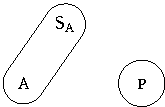
\includegraphics[width=0.3\linewidth]{figures/act_v_alignment}
	\begin{tikzpicture}
		\topnode{}
		\topleftnode[sa]{\gl{S\textsubscript{A}}}
	%	\toprightnode[sp]{\gl{s_p_}}
		\leftnode[a]{\gl{a}}
		\rightnode[p]{\gl{p}}
		\draw \convexpath{11.2pt}{a,sa};
		\draw (p) circle (11.2pt);
	\end{tikzpicture}
	\caption{Alignment for active verbs}
	\label{fig:alignment}
\end{figure}


\ea\label{ex:itr}
\gll le=soom\\
 3\gl{pl}=swim\\
\glt \qu{They swim.}
\z

\ea\label{ex:an}
\gll le=caihna li=apuli\\
  3\gl{pl}=know \gl{def}.\gl{pl}=person\\
\glt \qu{They know the people.}
\z


\ea\label{ex:stat}
\gll sinu-le\\
 suffer-3\gl{pl}\\
\glt \qu{They suffer.}
\z

%\begin{figure}
%	\centering
%	\begin{tikzpicture}
%	\topnode{}
%	\topleftnode[sa]{\gl{S\textsubscript{A}}}
%	\toprightnode[sp]{\gl{S\textsubscript{P}}}
%	%\leftnode[a]{\gl{a}}
%%	\rightnode[p]{\gl{p}}
%	%\align{sa, sp}
%	\single{sp}
%	\single{sa}
%	\end{tikzpicture}
%	\caption{Alignment for stative verbs}
%	\label{fig:alignment2}
%\end{figure}

%\textit{i sin xhopwen}
%und nicht wenn klar ist, wer gemeint ist

%\ea \ref{ex:v}
% 
% \ili{}{}{} Two active verbs, one in a matrix, one in a relative clause, with the same argument \textit{fati} \qu{speech, word} (B2:94)
% \gll e=holeke nya-si-m li=fati a \textbf{go}=vi
%  1\gl{sg}=receive put-hand-2\gl{sg} \gl{def}.\gl{pl}=speech \gl{rel} 2\gl{sg}=say
% \glt \qu{I gratefully receive from you the words you say}
% 
% \z 
 

A small class of stative verbs are formally indistinguishable from directly possessed nouns, except in that they don't take articles (\sectref{ssec:PossV}). Examples include \textit{mulip} \qu{life} \textit{muliv-am} \qu{you are alive}, \textit{hman-an} \qu{be hungry}.

\begin{table}
	\centering
	\caption{Subject and object markers for active and stative verbs}
	\begin{tabular}{lllll}
	\lsptoprule
		&	Free form	& \gl{a}=/\textsc{s\textsubscript{a}}= & -\textsc{s\textsubscript{p}} & -\gl{p}\\\midrule
		1\gl{sg} & \textit{io} & \textit{e} & \textit{-o(ng)} & \textit{-o} \\
		1\gl{du}.\gl{incl}& \textit{gasu} & \textit{gasu} & \textit{-gasu} & \textit{-kaeu}\\
		1\gl{pl}.\gl{incl} & \textit{gaa/gase} &\textit{ga(se)}&\textit{gaa}&\textit{-kaa}\\
		1\gl{du}.\gl{excl} & \textit{abu} & \textit{abu} & \textit{-abu} & \textit{-(a)bu}\\
		1\gl{pl}.\gl{excl} & \textit{abe}& \textit{abe} & \textit{-abe} & \textit{-(a)be}\\
		2\gl{sg} & \textit{go} &\textit{go} & \textit{-go} & \textit{-ko}\\
		2\gl{du} & \textit{gau} & \textit{gau} & \textit{-gau} & \textit{-kau}\\
		2\gl{pl} &\textit{gavwe}& \textit{gavwe} & \textit{-gavwe} & \textit{-kavwe}\\
		3\gl{sg} & \textit{ia} & \textit{a} & \textit{-(e)a} & \textit{-(e)a}\\
		3\gl{du} & \textit{lu} &\textit{lu} & \textit{-lu} & \textit{-lu}\\
		3\gl{pl} & \textit{le} & \textit{le} & \textit{-le} & \textit{-le}\\
	\lspbottomrule
	\end{tabular}
\label{tab:markers2}
\end{table}


\section{Impersonal verbs}
\label{sec:ZeroTrans}
\is{Verbs!Impersonal verbs}
Impersonal verbs, a term used by \textcite[70]{rivierre_langue_1980} for Cèmuhî, do not take argument indices and cannot occur in the imperative mood, but like other verbs they can form complete clauses by themselves and can either occur with an argument or without it. One subset of impersonal verbs, the affirmative existential \textit{vwa} and the negative existential \textit{cika}, can only take a noun phrase as an argument, but these are not the subject, as evidenced by their inability to take \textit{ka} \qu{\gl{sbj}}. This excludes pronouns. Since Vamale does not have a word for \qu{to have}, having or not having something is expressed with possessive constructions, as in (\ref{ex:vwa_have}): e.g. \qu{there is for me}, calqued into local French: \textit{Il y a une femme pour toi?} \qu{Is there a wife for you?} meaning \qu{Do you have a wife?} \textit{Cika} \qu{\gl{neg}.\gl{exist}} only takes inanimate and non-specific animate arguments, while \textit{cia-} is open to arguments of any animacy, and generic inanimates. \textit{Vwa} \qu{\gl{exist}} may exceptionally take free pronouns and specific animate arguments in marked scenarios (persons will usually be localized with \textit{la} \qu{be here} and demonstratives).

\ea \label{ex:vwa_have}\gll hê tha vwa li=xhaohmu vwa wadala-le\\
 yes \gl{ass} \gl{exist} \gl{def}.\gl{pl}=old \gl{exist} gun-3\gl{pl}.\gl{poss}\\
\glt \qu{Yes, there were elders who had guns.} {[KL:141]} 
\z

Another subset of impersonal verbs takes a complement clause as their sole argument (\ref{ex:impV1}), but can also stand alone (\ref{ex:impV2}). They form a small, closed class, partly derived from nouns. \textit{Goon ma} \qu{allowed, possible to}, \textit{vwasoon ma} \qu{impossible to},\footnote{Maybe from \textit{vwa-s(it)oon} \qu{\gl{exist}-taboo}.} \textit{siteke ma} \qu{forbidden to} work like this (see \Cref{fig:VwaTree}). 
Most members of this class have other meanings when used as nouns or verbs in other contexts, e.g. \textit{goon} \qu{body, enough} but \textit{goon, ma\ldots} \qu{possible, feasible, allowed to\ldots.}


\ea\label{ex:impV1}\gll vwasoon ma go=suu\\
 impossible \gl{comp} 2\gl{sg}=break\\
\glt \qu{You cannot break it.} {[AG1:71]}
\z

\ea\label{ex:impV2}\gll ju-vaa vwasoon\\
 very-too.much impossible\\
\glt \qu{It's too difficult.} {[KG:135]}
\z


%\a
% 
%\ili{}{}{} X10:7
%\gll th=e vwasoon
% \gl{ass}=1\gl{sg} impossible
%\glt \qu{I cannot}
%
%
%\a
%
%\gll *xhwan m=e vwasoon
% almost \gl{subr}=1\gl{sg} impossible
%\glt \qu{(It's almost impossible)}
%

%\ea\label{ex:xhwan}
%
%\ili{}{}{} X10:6
%\gll yo, xhwan ma vwasoon nyakoo-n m=e vwa ena
% 1\gl{sg} almost \gl{subr} impossible for-\gl{nspec} \gl{subr}=1\gl{sg} do \gl{dist} 
%\glt \qu{It's almost impossible for me to do this}
%

%e ra-xhwa thuang me caacaa
%e juu ra caacaa
%*e xhwathuang caacaa
%\qu{i am almost a father}

\textit{Uta} \qu{rain}, \textit{mapeke} \qu{be day}, \textit{bwen} \qu{night} and other members of the lexical field of weather phenomena, sea tide, etc. exist as article-bearing nouns as well, do not take arguments, but can form clauses and take certain adverbs. This third group is called verbs on the basis of constructions where the members cannot behave like typical nouns (\ref{ex:uta}), and following analyses of cognates in other languages, where the forms can be derived to take arguments: \textit{bwen-i-ɛg} \qu{It becomes night around me} \parencite[302]{rivierre_langue_1980}. This argument-taking is not attested in Vamale (anymore), but oblique constructions still exist.



	\ea \label{ex:uta}
		\gll (*i) uta nyako-ong\\
	 \gl{def}.\gl{sg} rain \gl{obl}-1\gl{sg}.\gl{poss}\\
	\glt \qu{It rains on me.}
	\z
	
	\ea	
	\gll thapoke mapeke\\
	 begin bright\\
	\glt \qu{It is (starting to) dawn.}
		\z



%The existential \textit{vwa} and the non-existential \textit{cika} are treated as stative verbs, though they cannot bear subject indices, which is perhaps explainable as a lexical semantic preference. 

%\subsection{vwasoon} %actually maybe not a verb. no agruments.

\begin{figure}
 \begin{forest}
		for tree={
			if n children=0{
				font=\itshape,
				tier=terminal,
			}{},
		}
		[S 
		[V[\textit{vwasoon}]]
		[S'[\textsc{subr}
		[\textit{ma}]]
		[VP
			[PN[\textit{go}{=}]]
			[,shape=coordinate
				[V [\textit{xaleke}]]
				[NP
					[ART[\textit{li}{=}]]
					[N[\textit{mani}]]
				]
			]
		]
		]
		]
	\end{forest}
	\caption{Tree-diagram of the sentence structure of \textit{vwasoon ma go xaleke li mani} \qu{You cannot see the birds}}
	\label{fig:VwaTree}
\end{figure}

%\begin{itemize}
%	\item \textit{vwasoon} \qu{difficult, impossible}
%	\item \textit{goon}\footnote{\textit{hmwagoon} \qu{be equal}} \qu{enough, permitted} this is derived from \textit{goo-n} \textit{body, size; zenith, maximum capacity}
%	\item \textit{vaang} \qu{unknown}
%	\item \textit{vwa} \qu{there is}
%	\item \textit{cika} \qu{there is not}
%	\item \textit{xhwat thuang} \qu{almost} is a fixed expression that takes no nominal argument and needs subordinate, possibly complement clause. it's not a verb since it takes no TAM.
%\end{itemize}
%\todo{are you sure this is only one class? cika wîîn but ?goon wîîn}

%\textit{Vwasoon} and \textit{goon} need a subordinator afterwards, which seems to be a clue that they do not take arguments. They are probably derived from nouns. \textit{goo-n xat} \qu{midday} looks like a classic possessive construction, literally \qu{enough sun} in the modern language, maybe \qu{maximal sun} before, because \textit{goon} is mostly used for \qu{enough, no more!} as a threat or plea, if it does not occur in the formula \textit{goon ma X...} \qu{it is possible/good...} (asking for permission or asking somebody to do something). \textit{Goon} also means \qu{body}. In the same sense, considering that the first syllable in \textit{vwasoon} \qu{impossible} only ever occurs as the morpheme \textit{vwa} \qu{exist; do}, this may be an old VP, lexicalized but still, following the "there is X" pattern, needless of arguments.
%\textit{Cika} \qu{\gl{neg}.\gl{exist}} is the same class as \textit{vwa} \qu{\gl{exist}}. They both take an argument, which can be implied if already mentioned.

 \section{Stative verbs}
\label{sec:StatV}
\is{Verbs!Stative verbs}

``Stative verbs" are a classic feature in New Caledonian languages, already described in \textcite{haudricourt_langues_1948}, and descend from Proto-Oceanic \parencite[63]{lynch_oceanic_2002}.\footnote{\citeauthor{lynch_oceanic_2002} distinguish stative and dynamic verbs, while the French tradition, and this study, call the latter ``active" verbs.} They are inflected with morphemes that closely resemble postponed free forms, as in \tabref{tab:hmet}. Like the undergoers of transitive verbs, the animacy of the referent decides whether the subject of a stative verb is marked: inanimate participants are not indexed on the verb.

\begin{table}
	\caption{Inflection of \textit{hmet-} \qu{sated}}
	\begin{tabular}{lll}
		\lsptoprule
\gl{sg} & 1 &\textit{hmet-eo}\\
		&2& \textit{hmet-go}\\
		&3& \textit{hmet-ea}\\
		\midrule
\gl{du} & 1\gl{incl}& \textit{hmet-gasu}\\
		&1\gl{excl}&\textit{hmet-abu}\\
		&2&\textit{hmet-au}\\
		&3& \textit{hmet-lu}\\
		\midrule
\gl{pl} & 1\gl{incl}& \textit{hmet-gaa}\\
		&1\gl{excl} & \textit{hmet-abe}\\
		&2 & \textit{hmet-gavwe}\\
		&3 & \textit{hmet-le}\\
		\lspbottomrule
	\end{tabular}
	\label{tab:hmet}
\end{table}

Stative verbs are a closed class, semantically vaguely characterized by a patientive S (though many active verbs also have a patientive S, e.g. \textit{weke} \qu{to be angry}, or \textit{khûda} \qu{to stink}). The argument is marked in the same position as transitive undergoers, and shares the latter's form, except in the first and second persons, where P arguments have a devoiced form, i.e. \textit{-ko} \qu{2\gl{sg}}, \textit{-kaa} \qu{1\gl{pl}.\gl{incl}} etc. This means that S is marked in two ways: S and A are marked the same for active verbs, and stative verb S subjects are either marked the same as P, or slightly differently, depending on the speaker and the verb. We thus have a tripartite system, though stative S and P are merged by many younger speakers, yielding a split-intransitive system like in western Voh-Koné. Diachronically, stative S and P participants were probably expressed as free pronouns following the predicate (V PN),\footnote{This may be linked to a Proto-Oceanic VSO or VOS word order \parencite[86, 87]{lynch_oceanic_2002}, though nowadays SVO is more widespread and considered canonic \parencite[49]{lynch_oceanic_2002}. Note that this would not explain the indexing found on active verbs.} which became incorporated into the verb (e.g. \textit{hmwet ia} \qu{tired 3\gl{sg}} $\rightarrow$ \textit{hmwet-ea}). Indirect possession underwent a similar process (\textit{thala-n ia} \qu{knife-\gl{poss} 3\gl{sg}} $\rightarrow$ \textit{thala n-ea}). 
The stative verb \textit{hmana-n} \qu{be hungry} (not a noun because it cannot take an article) has the paradigm of a directly possessed noun, and shares this property with \textit{muliva-n} \qu{be alive} (see \sectref{ssec:PossV}).

%\begin{itemize}
%	\item \textit{yamaan}\qu{be not motivated} 
%	\item \textit{saxhwe} \qu{refuse to eat} is actually just stative
%	\item \textit{sahnaang} \qu{not understand} is also just stative
%\end{itemize}


\subsection{Dependent stative verbs}
\label{ssec:Verbs_n}
\is{Verbs!Stative verbs!Dependent stative verbs}
Some verbs, active as well as stative ones, show nominal inflection. This grammar will use the term \textsc{dependent verb} found in some New Caledonian descriptions \parencite[207]{ozanne-rivierre_iaai_1976} for these verbs that can index a non-specific argument with a generic \textit{-n} (similarly to inalienably possessed nouns, called \textsc{dependent nouns} in the French tradition, which also cannot omit marking their modifier). Active verbs with nominal morphology work rather differently and are discussed in \sectref{ssec:active-n}. The verbs described here take different subject-indexing suffixes depending on animacy and specificity of the subject, as shown in \Cref{tab:V-n}. There are few still productive verbs in this category, but they are frequently used. Common members include \textit{xhopwe-n} \qu{grow/be big}, \textit{xhwati-n} \qu{be small}, \textit{hmai-n} \qu{be many}, \textit{sate-n} \qu{be different}, \textit{yape-n} \qu{be old (inanimate)}. % This section will use \textit{xhopwe} as an example.%, \textit{e-n} \qu{be first}. 


Animate subjects are indexed on stative verbs with personal suffixes (\textit{-eo} \qu{1\gl{sg}}, \textit{-go} \qu{2\gl{sg}} etc.) when they are not present as a noun phrase (\ref{ex:Vn1}). Inanimate subjects take \textit{-n} \qu{\gl{ana}} in these cases (\ref{ex:Vn2}). %If the subject is expressed as an NP in the same clause, the stative verb does not carry a suffix for animate NPs (\ref{ex:VnbareAnim}), and definite inanimate NPs (\ref{ex:VnbareInanim}). 

\ea\label{ex:Vn1}
\gll sate-o\\
 different-1\gl{sg}\\
\glt \qu{I am different.}
\z


\ea\label{ex:Vn2}
\gll sate-n (koo-n)\\
 different-\gl{ana} (\gl{obl}-\gl{ana})\\
\glt \qu{It is different (from it).}
\z

Generic subjects are always marked with \textit{-n} \qu{\gl{nspec}} (\ref{ex:Vn}). These rules begin to be less rigidly enforced in Voh-Koné languages in general \parencite[51]{rivierre_bwatoo_2006}, and \textit{-n} now often appears before noun phrases regardless of their animacy and specificity (\ref{ex:xhopwen i-X}). This may have contributed to the development of noun phrase internal modifiying verbs (see \sectref{sec:adj}).
\ea\label{ex:Vn}\gll e=vi hapi na naen xadaa sate-n \\
 1\gl{sg}=say \gl{comp} \gl{dem} now on.the.other.hand different-\gl{nspec}\\
\glt \qu{I'm saying that now things have changed.} {[KL:243]}
\z

Some stative verbs have split into two forms with different meanings, e.g. \textit{hmwaka-n}, \textit{hmwaka-o} \qu{be like it, be like me}, but \textit{hmwakan} \qu{maybe}.
Verbs with nominal morphology can also be found in Cèmuhî \parencite[179, 183]{rivierre_langue_1980} and Nyelâyu \parencite[48]{ozanne-rivierre_nyelayu_1998}. They are not described as an open class in these grammars. Though most verbs with nominal morphology in Vamale are stative, there are also active ones. A prominent example is \textit{caihna-n} \qu{to know} (discussed in more detail \sectref{ssec:active-n}). Some stative verbs with \textit{-n} can be derived with \textit{-ke} \qu{\gl{tr}}, compare \textit{xhwatii-n} \qu{be small} and \textit{xhwatii-ke} \qu{do softly}.







\begin{table}
	\caption{Meanings of \textit{xhopwe-} \qu{grow}}
	\begin{tabular}{lll}
	\lsptoprule
		1\gl{sg}	&\textit{xhopwe-o}& \qu{I grow}\\
		2\gl{sg}	&\textit{xhopwe-go}& \qu{You grow}\\
		3\gl{sg}&\textit{xhopwe-a}& \qu{S/He grows}\\
		\gl{nspec}& \textit{xhopwe-n} & \qu{It is big}\\
		overt NP & \textit{xhopwe} & \qu{It is bigger than X/before}\\
	\lspbottomrule
	\end{tabular}	
	\label{tab:V-n}
\end{table}

For \textit{xhopwe-n} \qu{big}, there is a meaning distinction along an animacy axis: without \textit{-n}, it expresses either a development \qu{big} $\rightarrow$ \qu{get bigger}, through time in comparison with an earlier state (\qu{grow}), or synchronically in comparison with others (\qu{be bigger than}, see example \ref{ex:VnAnim}). A table summarizes the forms (\Cref{tab:V-n}). \textit{xhopwe-} means \qu{to be bigger} for animate subjects (\ref{ex:VnAnim}) and \qu{to be big} for inanimates (\ref{ex:xhopwen i-X}, \ref{ex:xhopwen}). %, if it is clear from the context that it is a momentary observation. %\textit{xhopwe-} means \qu{to grow, to be bigger} for all subjects (\ref{ex:VnbareInanim}, \ref{ex:xhopwen can}). 


\ea\label{ex:VnAnim}\gll 	i=apuli a= xhopwe-a (koo-le)\\	
	\gl{def}.\gl{sg}=man \gl{rel}= big-3\gl{sg}.\gl{S\textsubscript{P}}	(\gl{obl}-3\gl{pl})\\
	\glt	\qu{the bigger man (in years, status, size) (than them)}	\\
\z

\ea\label{ex:xhopwen i-X}
\gll 	xhopwe(n) i=goon	\\
	big	\gl{def}.\gl{sg}=body\\
\glt	\qu{the big body (height, corpulence)}
\z
%\a
%
%\gll 	*xhopwen goon	
%	big body	
%%\glt	personne de grande taille	
%
%\a\label{ex:VnbareInanim}
%
%\ili{}{}{} \textit{xhopwe-n} and other verbs denoting amount, size, length etc take comparative meaning in appropriate settings.
%\gll 	xhopwe i si-n mo-ko i s-ung	
%	big \gl{def}.\gl{sg}=hand-3\gl{sg}.\gl{poss} more.than \gl{def}.\gl{sg}=hand-1\gl{sg}.\gl{poss}	
%\glt	\qu{His hand is bigger than mine}	
%

%\textit{xhopwen} in (\ref{ex:xhopwen i-X}) means \qu{its growth, its size}, and is derived from \qu{to grow}. Compare \textit{hun-xhopwen an}, literally \qu{his/her way of being/becoming big} means \qu{his/her corpulence}. % %todo{??? What is exactly derived from what here...?} 
%though
%Syntactically, \textit{xhopwen} is used similarly to \textit{joaka-n}, as shown in \Cref{tree:joakan}, .
A construction frequently seen with animate subjects is shown in (\ref{ex:xhopwen}). The unmarked use of \textit{xhopwe}, as explained above, is as a predicate with comparative meaning (\ref{ex:VnbareAnim}). In a relative clause, \textit{xhopwe} is ungrammatical without a resumptive subject-indexing suffix (\ref{ex:Vno}), e.g. \textit{-a}, or an anaphoric suffix \textit{-n} (\ref{ex:xhopwen can}). In example (\ref{ex:xhopwen}), however, the meaning of \textit{xhopwen} is not comparative. This construction seems to be a strategy to avoid the incremental\slash comparative meaning of certain stative verbs, and may be related to the de\hyp grammaticalization of \textit{-n} mentioned for \textit{xhopwen} in \Cref{tab:V-n}.


\ea[]{\label{ex:xhopwen}
%\ili{}{}{} This seems to be an expression, where the \textit{-n} refers not to the man, but to his body.
\gll 	i=apuli a= xhopwe-n\\
	\gl{def}.\gl{sg}=man \gl{rel}= big-\gl{ana}	\\
\glt	\qu{the fat/old/important man}}
\z


\ea[]{\label{ex:VnbareAnim}
\gll 	xhopwe i=apuli-aen	\\
	grow \gl{def}.\gl{sg}=man-\gl{dem}	\\
\glt	\qu{This man is bigger/taller/ more important.}}
\z

\ea[*]{\label{ex:Vno}
\gll 	i=apuli a= xhopwe\\
	\gl{def}.\gl{sg}=man \gl{rel}= big	\\
\glt	(for: \qu{the man who is big})}
\z

\ea[]{\label{ex:xhopwen can}\gll 	i=apuli a= xhopwe-n ca-n dawee-lu	\\
	\gl{def}.\gl{sg}=man \gl{rel}= big-\gl{ana} in-\gl{nspec} between-3\gl{du}.\gl{poss}	\\
\glt	\qu{the fatter man of the two}}	
\z

	%\a
	%
	%%% \ili{}{}{} 
	%\gll 	*si-n xhopwen	
	%		
	%\glt		
	%
	
	%\a
	%
	%%% \ili{}{}{} 
	%\gll 	si-n a xhopwen	
	%	hand-3\gl{sg}.\gl{poss} \gl{rel} big	
	%\glt	\qu{(The) hand which is big}
	%
%	\z
	
%\end{multicols}


%\begin{table}
%	\label{tab:V-n}
%	\caption{V-n}
%\begin{tabular}{lllll}
%
%Verb & \gl{def} hand & \gl{indf} hand & \gl{def} man & \gl{indf} man\\
%\midrule
%xhopwe \_ & the hand is big & * & the biggest & an elder\\
%vaa xhopwe \_ & the biggest hand& * & the biggest & an elder\\
%%\_ a xhopwe & * & * & * & *\\
%%\_ xhopwe & * & * & * & *\\
%xhopwen \_ &the big hand &* &* &*\\
%%xhopwen \_ & & *vuki yee &&\\
%\_ a xhopwen & the big hand & size & the big man & a big man\\
%\_ xhopwen & i sin & sin & size & size \\
%\_ a kon xhopwen & i sin & sin & * & * \\
%%\midrule
%xhopwea\_ & * & * & he gets fatter & *\\
%\_ a xhopwea & * & * & the elder/biggest & the elder/biggest \\
%\_ xhopwea & &&elder&elder \\
%\_ a kon xhopwea & * & * & growing&\\
%\_ a kon xhopwen & & & growing? & \\
%\midrule
%cie\_ & * &* & i/eca apuli & *\\
%\_ cie-a & * & * & the/some man is absent & *\\
%cian & the hand is not there&*&*&* \\
%\end{tabular}
%\end{table}

%Hypothesis: animacy plays a role, it's not productive anymore (otherwise daahma a xhopwen would not work) or xhopwen is special.


\subsection{Numerals}
\label{ssec:Numerals}
\is{Numerals}
\is{Verbs!Numerals}

Numerals in Vamale are stative verbs that can take subject suffixes, as \Cref{tab:numbers} shows. Some are derived from nouns, notably 5 from \qu{hand}\footnote{From \textit{si-} \qu{hand}, showing the tendency to rather speak of 2\gl{sg} or 1\gl{pl}.\gl{incl} than an indefinite 3\gl{sg}.} and 20 from \qu{person}, the bases of the system. Complex numerals used to be formed like clauses, made of coordinated verb phrases. 

%\begin{minipage}{\textwidth}
\begin{table}
	\centering
\caption{The first six cardinal numerals and their verbal form}
\begin{tabular}{llll}
\lsptoprule
Number & Gloss & Suffixed form & Gloss\\\cmidrule(r){1-2}\cmidrule(l){3-4}
\textit{se}& \qu{1}& \textit{see-a} & \qu{s/he is one, s/he is alone}\\
\textit{thalo(o)}& \qu{2} & \textit{thaloo-lu} & \qu{they are two}\\
\textit{thi(i)en}& \qu{3} & \textit{thien-le} & \qu{they are three}\\
\textit{fava}& \qu{4}& \textit{fava-le} & \qu{they are four}\\
\textit{nim} & \qu{5}& \textit{nim-le} & \qu{they are five}\\
\textit{nim a bwa se}& \qu{6}& \textit{nim a bwa see-le} & \qu{they are six}\\
\lspbottomrule
\end{tabular}
\label{tab:numbers}
\end{table}
%\end{minipage}


 \textit{(N)a-bwa} was only recorded with complex numerals, some of which are shown in \Cref{tab:compo_numbers}. The initial nasal only occurs if the preceding element ends in an open syllable. Bwatoo has \textit{bwa} as \qu{+} \parencite[45]{rivierre_bwatoo_2006}, maybe related to \textit{pwa} \qu{on} or \textit{bwa}- \qu{head}. Leenhardt translates \textit{vajilu ka bwa nim ka bwa se} \qu{16}, then with \textit{ka} instead of \textit{na}, as \qu{ten and the right hand raised and open, and the thumb sticking out of the fist}, but no modern Vamale word would tie \textit{bwa} to either palm (\textit{yataan}), fist (\textit{daamuun}) nor the right hand (\textit{juu sin}) \parencite[166]{leenhardt_langues_1946}. The element having replaced the coordinator \textit{ka} is another puzzle. The demonstrative pronoun \textit{na} often means \qu{It is X (who did/is Y)}, and may have replaced the former coordinator \textit{ka} \parencite[166]{leenhardt_langues_1946} in a sense of `five, this on top of two' for \qu{7} (\ref{ex:7}). This grammar writes the coordinator \textit{na-bwa} joined by a hyphen to account for its single stress contour.
 
\ea \label{ex:7}
 \gll nim (a)-bwa thaloo\\
	  5    plus   2\\
 \glt \qu{7}\\
 \z 

\begin{table}
	\caption{Complex numerals}
	\begin{tabular}{ll}
	\lsptoprule
		\textit{vajilu na-bwa nim a-bwa se} & \qu{16}\\
		\textit{thaloo vajilu} & \qu{20}\\
		\textit{se apuli} \textit{na-bwa nim a-bwa se}& \qu{26}\footnote{\textit{se apuli} lit. \qu{one person}}\\
		\textit{se apuli na-bwa vajilu}& \qu{30}\\
		\textit{thaloo apuli}& \qu{40} (arch.)\footnote{This is never given spontaneously. People are mentally in a ten-based system now (see the word for 20).}\\
		\textit{nim apuli}& \qu{100} \\
		\textit{apuli ko apuli} & \qu{400}\\
	\lspbottomrule
	\end{tabular}
	\label{tab:compo_numbers}
\end{table}

\textit{Vajilu} \qu{10} could be etymologically composed as in (\ref{ex:10}). The last syllable is likely \textit{-lu} marking 3\gl{du}.\gl{poss} on nouns. The system being 5-and 20-based as is typical of the region \parencite[261]{haudricourt_dictionnaire_1982}, and finally \textit{Iaai} saying \qu{two hands} for 10, maybe the etymology of this word is something like in (\ref{ex:10}), but this is purely speculative.

\ea \label{ex:10}
\gll vwa si-lu\\
 \gl{exist} hand-3\gl{du}.\gl{poss}\\
\glt \qu{They have hands/there are their hands.}
\z 

According to \textcite[45]{rivierre_bwatoo_2006}, and also Dego Philippe Gohoupe, another word for 100 is \textit{se apuli} \qu{one person}. This confusing polysemy makes more sense considering that the Pacific Franc used to have a 100 Franc bill with a man on it (see \Cref{fig:100CFP}), was a salient thing, and spoken about much more often than groups of twenty. Nowadays, saying \textit{se apuli} normally means \qu{100}, but \textit{se apuli na bwa se} is \qu{21}, whereas \textit{nim apuli} is \qu{100} if it is part of a complex numeral. Leenhardt notes \textit{nilu apuli} for \qu{100} without glossing it \parencite[166]{leenhardt_langues_1946}{}. Whether \textit{nim apuli} is interpreted as 500 or 100 is difficult to ascertain, since most speakers are unsure. Vamale numerals are rarely used beyond 5 in the language, while French loans are taking over due to school, money, hours of the day, and a decay of counting contributions in customary ceremonies. Multiplying based on 20 is attested in \citetitle{leenhardt_langues_1946} for most languages, amongst which is Hmwaveke with \textit{sec apulip ko apulip} for 400, literally \qu{one person on people, or \qu{20 on 20}}, which suggests, along with \textit{nim apuli} \qu{100 (lit. 5 20)}, that the multiplication base comes last, and the multiplier first \parencite{leenhardt_langues_1946}. 

\begin{figure}
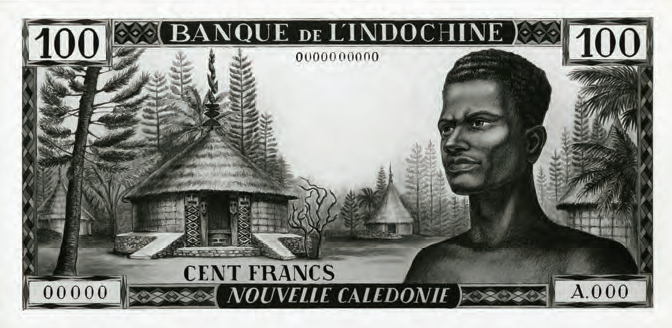
\includegraphics[width=\linewidth]{figures/100_francs}
\caption{A 100 CFP bill from 1964 \parencite[24]{ieom_lhistoire_2014}}
	\label{fig:100CFP}
\end{figure}
 
\subsubsection{Ordinals}
\is{Ordinals}
\is{Verbs!Ordinals}
\largerpage

Ordinals are formed with \textit{e-}\footnote{\textit{bɛ-} in Cèmuhî, used only with ordinals  \parencite[271]{rivierre_langue_1980}.} and \textit{(k)a-n} \qu{\gl{clf}.\gl{poss}-\gl{nspec}},\footnote{The Cèmuhî cognate [hɛ̃̀] is analyzed as a possessive morpheme by Rivierre \parencite[271]{rivierre_langue_1980} and otherwise only present in part-of-whole compounds.} yielding the forms listed in \Cref{tab:ordinal}. Leenhardt (1946) recorded irregular forms which have now disappeared, \textit{i a vathabun} \qu{the first (lit. s/he who is in front)},\footnote{Leenhardt's \textit{vathabun} is \textit{pa(a)thabun} nowadays.} now regular \textit{i e-se=kan} \qu{the first}, and \textit{i ethice nawe},\footnote{Since the clitic \textit{=(k)a-n} is used for possessum classifying purposes elsewhere, Leenhardt's form could have been \textit{i e-thicen=a-vwe}, with -\textit{vwe} \qu{2\gl{pl}.\gl{poss}}.} now \textit{i e-thien=an}. They, too, are rarely used beyond 5.

\begin{table}
	\caption{Ordinals}
	\begin{tabular}{ll}
	\lsptoprule
		\textit{(i) e-se kan} & \qu{(the) first}\\
		\textit{i e-thalo kan} & \qu{the second}\\
		\textit{i e-thien an} & \qu{the third}\\
		\textit{i e-fava kan}&\qu{the fourth}\\
		\textit{i e-nim an}&\qu{the fifth}\\
		\textit{i e-vajilu na bwa nim na bwa se kan}&\qu{the sixteenth}\\
		\textit{i e-koin an}& \qu{the last}\\
	\lspbottomrule
	\end{tabular}
	\label{tab:ordinal}
\end{table}

Ordinal numbers seem to have lexicalized \textit{ka-n} \qu{\gl{clf}.\gl{poss}-\gl{nspec}}, since it cannot be omitted. Onto it, another \textit{ka} can be added (but does not necessarily have to be) in order to make it possessible by the noun \textit{en} \qu{moment} (\ref{ex:kan en}, \ref{ex:kan en2}).

\ea \label{ex:kan en}\gll ja i={\ob}e-thalo-kan ka-n en{\cb} a tipwa\\
 \gl{prf} \gl{def}.\gl{sg}=\gl{ord}-two-\gl{link} \gl{clf}.\gl{poss}-\gl{nspec} moment \gl{rel}.3\gl{sg} fall\\
\glt \qu{It is the second time that it falls.} {[JN1:21]}
\z


\ea \label{ex:kan en2}
%\ili{\textit{ja iekoinan kan en exaleko}}\\
\gll ja i=e-koin-an ka-n en a= e=xale-ko\\
 \gl{prf} \gl{def}.\gl{sg}=\gl{ord}-end-\gl{link} \gl{clf}.\gl{poss}-\gl{nspec} moment \gl{rel}= 1\gl{sg}=see-2\gl{sg}.\gl{obj}\\
\glt \qu{It is the last time that I saw you.} {[JN1:36]}
\z


\subsubsection{Multiplicative \textit{o}}
\is{Numerals!Multiplicative}

The multiplicative prefix \textit{o-} (\qu{X times}) only occurs with numerals. The resulting word is derived to an adverb (\ref{ex:o-thiien}). Hence, multiplicatives cannot be predicates in a matrix clause, but do occur in adjunct clauses. Exceptions are interjections like the work call \textit{o-see!} \qu{do at once, in one hard pull}. \textit{O} \qu{X times} is analyzed as a prefix as well in Nêlêmwa \parencite[39]{bril_nelemwa_2002} and Bwatoo (where it is \textit{we-}) \parencite[46]{rivierre_bwatoo_2006}. In (\ref{ex:hunmata}), however, the adverb is possessed by a third person. I analyze this as a zero derivation.

\ea\label{ex:o-thiien}
\gll a=tho nyakoo-m \textbf{o-thiien} \\ %\textsubscript{Adjunct}
 3\gl{sg}=call \gl{obl}-2\gl{sg}.\gl{poss} times-three\\
\glt \qu{S/he called you three times.} {[2019-08-05 JP ka 42.1]}
\z


\ea\label{ex:hunmata}\gll pa ja o-thien-n-ea ko i=(hun-) mata\\
 \gl{prf} \gl{prf} times-three-\gl{poss}-3\gl{sg}.\gl{poss} \gl{obl} \gl{def}.\gl{sg}=\gl{nmlz}- sing\\
\glt \qu{This is the third time that he sings.} {[vamale-181127-jp\_nelemwa-1: 00:11:51-00:11:52]}
\z


%\ea
%\begin{multicols}{2}
%	\a
%	
%	\ili{}{}{} PE1:22.1 Is this really the same?
%	
%	\gll {[}{[}nim-ambwa-see]\textsubscript{V} o]\textsubscript{Adverbial Clause} {[}hun-bita-eo]\textsubscript{NP}
%	
%	 5-plus-1 times \gl{nmlz}-turn-1\gl{sg}
%	
%	\glt \qu{6 times I turned}
%	
%	
%	
%	
%	\a
%	
%	\gll nim-ambwa-see\textsubscript{V} o hun-bita-eo
%	
%	 5-plus-1 \gl{irr} \gl{nmlz}-turn-1\gl{sg}.\gl{poss}
%	
%	\glt \qu{Six would be my turns}
%	
%	
%\end{multicols}
%\z
%\todo{listen to the recording} 


\subsection{Possessible verbs}
\label{ssec:PossV}
\is{Verbs!Possessible verbs}

``Possessible verbs" are distinguished here from ``verbs with \textit{-n}", though they both carry a morpheme \textit{-n} in the third person, because the latter inflect using stative subject indexing suffixes (including \textit{-n} \qu{\gl{nspec}}), and the former take possessive morphology (including \textit{-n} \qu{3\gl{sg}.\gl{poss}}, see \Cref{tab:poss}). There are two subsets of stative possessible verbs, one with alienable and one with inalienable possessive morphology. 
Inalienably possessed intransitive verbs, such as the ones below (\ref{ex:hman1}), are not transparently derived from nouns (\ref{ex:hman3}), with the exception of \textit{nyima-} \qu{heart} \goodtilde \qu{to want}. Nouns can be derived from some of them using typical deverbal constructions (\ref{ex:xhopwen i}).
\begin{enumerate}[(a)]
\item \textit{hman-ong} \qu{I am hungry}, \textit{hmana-n}  \qu{s/he is hungry}
\item \textit{bwaa-ng}, \textit{bwaa-n}, \textit{bwaa-ju} \qu{if only}. This has an interjection counterpart \textit{bwaa-m} \qu{poor/darling you!}. Since this item cannot take an article and can stand as clause, it is analyzed as a verb.
\item \textit{holoo-m}, \textit{holoo-u}, \textit{holoo-vwe} \qu{goodbye (you, you two, you all)}
\item \textit{nyim-ong} \qu{I want, like}
\item \textit{vwaseek-ong} \qu{I am sad}
\end{enumerate}


	
	\ea\label{ex:hman1}
	% \ili{}{}{} \textit{hmanong}, \textit{hmanam}, \textit{hmanan}
	\gll hman-ong\\
	 hungry-1\gl{sg}.\gl{poss}\\
	\glt \qu{I am hungry.}
	\z
	% *i sinuong %that's just a normal stative verb, what the fuck
%	\ea\label{ex:hman2}
%	
%	\gll *i=hman
%	 \gl{def}=hunger
%	\glt (for: \qu{The hunger})
%	
	
	 \ea\label{ex:hman3}
	     \textit{*i=hman-an} (for: \qu{his/her hunger})
	\z
	
	\ea\label{ex:xhopwen i}
	\gll paa juu va xhopwen i=hun-hman-ong\\
	 already really too big \gl{def}.\gl{sg}-\gl{nmlz}-hungry-1\gl{sg}(.\gl{poss})\\
	\glt \qu{I am more and more hungry.} (lit. \qu{My hungering has become really big})
\z
	% \a
	% 
	% \gll i=nyai-n
	%  \gl{def}=offspring-3\gl{sg}.{poss}
	% \glt \qu{his/her child {[}inalienable]}
	% 
	


There are few alienably possessed intransitive verbs. They include \textit{yamaan-eong}, \textit{yamaan-ea}, \textit{yamaan-gasu} \qu{be unwilling to do for lack of motivation, be fed up with something}, and \textit{saxhwe-ong}, \textit{saxhwe-a} \qu{refuse to do},\footnote{This possibly contains the morpheme \textit{xhwe} \qu{be across}.} as well as \textit{yathô-ong}, \textit{yathô-a} \qu{be in a hurry}. \textit{Sinu-ong}, \qu{be sick, be suffering; die} also exists as a noun meaning \qu{illness}. % is indistinguishable from stative verbs except in the first person, there is some flexibility.
Possessible verbs, mostly verbs with an Undergoer argument, take possessive morphology usually found on nouns, but cannot bear an article. They are intransitive, like all stative verbs. The second subset, with alienable possessive morphology, could be derived from the very similar stative paradigm, and in many cases the subject-indexing suffixes differ between speakers: \textit{sino-ong} \goodtilde \textit{sinu-o} \qu{ill-1\gl{sg}}, \textit{saxhwe-ong} \goodtilde \textit{saxhwe-o} \qu{refuse-1\gl{sg}}.

 \section{Active verbs}
 \label{sec:ActV}
 \is{Verbs!Active verbs}
Active verbs, the biggest group of verbs, have transitive and intransitive members, and many of them are ambitransitive, meaning they can take an object, but do not have to. As is common in Oceanic languages \parencite[510]{ross_morphosyntactic_2004}, there are no ditransitive verbs in Vamale. This section will first introduce transitive verbs, with their suffixes \textit{-i} and \textit{-ke}, then describe transitive verbs with nominal inflection (called \qu*{dependent} transitive verbs), before addressing transitive verbs that require a preposition \textit{ko-} \qu{on}.

Active intransitive verbs are formally not distinct from transitive verbs, except in that they do not take object suffixes. This is in line with Proto-Oceanic \parencite[81]{lynch_oceanic_2002}. Both transitive (e.g. \textit{vavi} \qu{hunt something}) and ambitransitive verbs (e.g. \textit{xaahni} \qu{check, stare (at)}) can occur without an argument, before other (ad)verbal elements of the verb phrase, or with a generic argument, and will still carry transitive suffixes \textit{-i} or \textit{-ke}, discussed below. Purely intransitive ones usually do not end in \textit{-i} or \textit{-ke}, see (\ref{ex:intrV}). All active verbs take subject marking bound pronouns, as in examples (\ref{ex:index_actV}) and (\ref{ex:index_actV2}). \Cref{tab:markers2} lists the bound pronouns.

\ea \label{ex:intrV}\gll tabo tabo li=xho thamo, thêên thêên li=xho xayu\\
 sit sit \gl{def}.\gl{pl}=cicada female fly fly \gl{def}.\gl{pl}=cicada male\\
\glt \qu{Sit sit oh female cicadas [full of eggs], fly fly (away) oh male cicadas.} (children's song, female cicadas bear eggs and are tastier) {[children's song]}
\z

\ea \label{ex:index_actV}\gll \textbf{e}=han-mwa ko-m=\textbf{e} vwa ma=\textbf{a} thuup ka i=jamw-ong\\
 1\gl{sg}=go-\gl{rep} because-\gl{subr}=1\gl{sg} do \gl{comp}=3\gl{sg} bathe \gl{sbj} \gl{def}.\gl{sg}=father-1\gl{sg}.\gl{poss}\\
\glt \qu{I'm going back to make my father take a bath.} {[PQ 10.1]}
\z


\ea \label{ex:index_actV2}\gll tha=\textbf{abe}=vataan fai li=ya-be. cahma li=mama-n-abe, \textit{non}. tha=\textbf{le} fwi-kabe ma=\textbf{abe}=mu bwa e-nyoot\\
 \gl{ass}=1\gl{pl}.\gl{excl}=each cook \gl{def}.\gl{pl}=starchy.food-1\gl{pl}.\gl{excl} concerning \gl{def}.\gl{pl}=mother-\gl{poss}-1\gl{pl}.\gl{excl} no \gl{ass}=3\gl{pl} pinch-1\gl{pl}.\gl{excl}.\gl{obj} \gl{subr}=1\gl{pl}.\gl{excl}=\gl{freq} \gl{ipfv} \gl{refl}-wake.up\\
\glt  \qu{We'd cook our own lunch. Our mothers however, no. They'd pinch us so that we'd wake up.} {[PE2:50]}
\z

\subsection{Transitive verbs}
\label{ssec:TransV}
Transitive verbs mark the subject at the beginning and the undergoer object (if animate, but this condition is disappearing) at the end (\ref{ex:actV}).\footnote{In example \REF{ex:actV}, the subject marker was omitted. This may be due to the elicitation context, where there no referent for the chaser was established. } There are no ditransitive verbs; non-core arguments such as recipients, goals, experiencers and stimuli (depending, of course, on the verb) are marked with the oblique markers \textit{nyasi-} and \textit{nyako-} (see \sectref{sec:oblique}). The transitive verb \textit{holeke} \qu{thank, receive}, for example, has the Theme as a direct object and the Recipient is added through \textit{nyako}- or \textit{nyasi}- (\ref{ex:nyasi_bofukaje}). \textit{nyasi}- is more polite and can only be used with humans. Transitive verbs almost invariably appear with the now lexicalized transitive suffix \textit{-i}, \is{Transitivity!Transitive \textit{-i}}\is{Transitivity!Transitive \textit{-ke}}possibly descended from Proto-Oceanic \textit{*-i} \parencite[507]{ross_morphosyntactic_2004}, or with the still productive \textit{-ke}, possibly descended from \textit{*-akin(i)} \parencite[507]{ross_morphosyntactic_2004}. \sectref{ssec:ke_i} describes this in more detail. Transitive verbs without these suffixes are e.g. \textit{tua} \qu{detach}, \textit{tuu} \qu{take something out of somewhere}, \textit{sivu} \qu{blow; smoke}.

\ea \label{ex:actV}\gll (a=) ha-me wati-ko ko go=imwi i=nyai-n\\
 3\gl{sg}= go-\gl{dir.cp} chase-2\gl{sg}.\gl{obj} because 2\gl{sg}=grab \gl{def}.\gl{sg}=child-3\gl{sg}.\gl{poss}\\
\glt \qu{It comes to chase you because you took its pup.} {[B2:36]}
\z

\ea \label{ex:nyasi_bofukaje}\gll gaa=se-me holeke \textbf{nyasi} bofukaje i=thoatit-ca a= tha=a=bwa nya si-je\\
 1\gl{pl}.\gl{incl}=together thank \gl{obl} god \gl{def}.\gl{sg}=day-\gl{dem}.\gl{prox} \gl{rel}= \gl{ass}=3\gl{sg}=\gl{ipfv} put \gl{ben}-1\gl{pl}.\gl{incl}\\
\glt \qu{We all thank God together for this day that he gave us.} {[Adèle Gohoupe's Song ``Hole Nyasi Daahma":1]}
\z 



%\ex 
%
%\ili{}{}{} GD:12
%\gll  ma xa-wekee-go, go feana-ke ca wîî-m, go hân cabi doop! e=bo \textbf{cade-ko}, go eca apuli
%
% \gl{subr} \gl{agt}.\gl{nmlz}-rage-2\gl{sg}, 2\gl{sg} show-\gl{appl} \gl{indf}.\gl{pl} strength-2\gl{sg}.\gl{poss}, 2\gl{sg} go crush soil 1\gl{sg} \gl{irr} admire-2\gl{sg}.\gl{obj} 2\gl{sg} \gl{indf}.\gl{sg}=person
%
%\glt \qu{If you are enraged, show your strength, go break{ [=}till] some earth ! {[Then]} I shall admire you, {[}if] you are a man.}
%
%
%\z

\subsubsection{Transitive suffixes \textit{-ke} and \textit{-i}}
\label{ssec:ke_i}
\is{Transitivity!Transitive \textit{-ke}}
The transitive suffix -\textit{ke} is the only productive transitive suffix in Vamale. This grammar calls \textit{-ke} a transitive rather than applicative suffix because it does not routinely turn obliques into direct objects, but can derive transitive from intransitive verbs, or even transitive verbs from complex verbs and nouns. Furthermore, and perhaps most importantly, the suffix is in complementary distribution with an object marker: \textit{-ke} appears if the animate object is not overt, as in examples (\ref{ex:ke_noke1}) and (\ref{ex:ke_noke2}). This distiguishes \textit{-ke} from \textit{-i}, which is part of the stem and cannot be replaced.\footnote{Contrary to the Vamale form \textit{-ke}, the Cèmuhî cognate {[}-hĩ] can derive stative and impersonal verbs such as {[}tìtì] \qu{wet} (Vam. \textit{titi}) \qu{to be likely to wet something} and [ūtɛ̄] \qu{rain} (Vam. \textit{uta}) to {[}ūtɛ̄-hĩ] \qu{to be rained upon} \parencite[255]{rivierre_langue_1980}.} Note that both \textit{-ke} and \textit{-i} (described further down) likely have Proto-Oceanic origins, \textit{*-akin(i)} and \textit{*-i}, respectively \parencite[507]{ross_morphosyntactic_2004}, though the latter are reconstructed as applicative suffixes. 



	\ea\label{ex:ke_noke1}	
	\gll le=xhiile-a\\
	 3\gl{pl}=flog-3\gl{sg}.\gl{obj}\\
	\glt \qu{They flog him/her.}
	\z
	
	
	\ea\label{ex:ke_noke2}
	\gll le=xhiile-ke i=apuli\\
	 3\gl{pl}=flog-\gl{tr} \gl{def}.\gl{sg}=person\\
	\glt \qu{They flog the person.}
		\z


%, but sometimes the transitivity of the verb is clear in total absence of an idea of the object, its number etc (). 
%\textit{xaleke?} \qu{see?} is a common discourse marker and elicits a minimal response, can take an object, but does not have to. 
Most verbs that take \textit{-ke} and (still) have a counterpart without the suffix, are active verbs, as \Cref{tab:ke} shows. For example, the verb \textit{xaleke} \qu{to look at something, to see something} has two sisters that also relate to visual intake: \textit{xale} \qu{to look without clear purpose} is either intransitive and means \qu{to look around}, or means \qu{to visit} and takes animate undergoers (\ref{ex:xale}).

\ea \label{ex:xale}\gll i=se a= lu=mee hup-e ya a=bwa ta xale\\
 \gl{def}.\gl{sg}=other \gl{rel}= 3\gl{du}=all go.down-\gl{dir.cp} 3\gl{sg} 3\gl{sg}=\gl{ipfv} go.up look\\
\glt \qu{The other who came with (lit. the other that the two came down together) went up [in the gas station] to look around.} {[KG:471]}
\z

\begin{sloppypar}
\textit{Xalo koo-n} \qu{gaze (at something, with no implication of understanding or recognition)} illustrates another way of expressing transitivity: with \textit{ko} \qu{\gl{obl}} (see \sectref{ssec:koon}). \textit{Xhaavwa koo-n} \qu{wait around for it} is the less transitive counterpart to \textit{xhavwaleke} \qu{await}, possibly because \textit{xhavwale} would look like a transitive 3\gl{pl} object verb. Another possibility would be an older form \textit{xhwaavwat} that eventually dropped the last plosive to yield modern \textit{xhaavwa}. This would be similar to \textit{sesaat} \qu{sneak}, \textit{sesaaleke} \qu{stalk}. %Pije te-hyaakhô
The suffix -\textit{ke} is not reserved for animate objects, as \textit{feanake} \qu{to show} illustrates in example (\ref{ex:feanake}): if the animate undergoer is present as a noun phrase, \textit{-ke} remains, otherwise the undergoer is indexed via a suffix (\ref{ex:feanaa}).% , \textit{holeke} \qu{to thank for, receive}, \textit{xhateeke}\footnote{Possibly from \textit{xat} \qu{sun}. \textit{xhat} \qu{clitoris} seems an unlikely root.} \qu{to dry something} show. 
\end{sloppypar}


\ea\label{ex:feanake}
\gll feana-ke i=si-m, feana-ke i=thamo!\\
 show-\gl{tr} \gl{def}.\gl{sg}=hand-2\gl{sg}.\gl{poss} show-\gl{tr} \gl{def}.\gl{sg}=woman\\
\glt \qu{Show your hand, show the woman {[}e.g. to me]!}
\z


\ea\label{ex:feanaa}
\gll feana-a!\\
 show-3\gl{sg}.\gl{obj}\\
\glt \qu{Show him/her!}
\z

%Since these verbs end with -\textit{ke} but are not used with animate objects, maybe -\textit{ke} has other functions too?


\begin{table}
	\caption{Pairs with and without \textit{-ke}}
	\begin{tabular}{llll}
		\lsptoprule
		Verb & With overt anim. P & With pronoun & With overt inan. P\\\midrule
		\textit{xale} & \textit{xale i apuli} & *\textit{xale yo, xale go} & *\textit{xale i mwa}\\
		`visit, look  & \qu{go see the person} & &  \\
		\quad around' & \\
		\addlinespace
		\textit{xaleke} & \textit{xaleke i apuli} & \textit{xale-o, xale-ko} & \textit{xaleke i mwa}\\
		\qu{see} & \qu{see the man}& \qu{see me, see you} & \qu{see the house}\\
		\addlinespace
		\textit{cade} & \textit{cade i apuli} & *\textit{cade-go}& *\textit{cade i mwa} \\
		\qu{admire} & \qu{admire the man} & & \\
		\addlinespace
		\textit{cadeke} & \textit{cadeke i apuli} & \textit{cade-ko} & \textit{cadeke i mwa}\\
		\qu{admire} & \qu{admire the man} & \qu{admire you} & \qu{admire the house}\\
		\addlinespace
		\textit{vathân} & \multicolumn{3}{l}{is a preverb (see \Cref{ssec:Preverbs})} \\
		\qu{do separately}& & & \\
		\addlinespace
		\textit{vathânke} & \textit{vathânke li=apuli} & \textit{vathân-le} & \textit{vathânke i we} \\
		\qu{separate} & \qu{separate the men} & \qu{scatter them} & \qu{part the water}\\
		\lspbottomrule
	\end{tabular}
\label{tab:ke}
\end{table}

\textit{-ke} is also used with the stative verb \textit{xhwatii-n} \qu{be small},  yielding \textit{xhwatiike} \qu{do softly}, as in (\ref{ex:xhwatiike}). Note that \textit{xhwatiike}, despite the translation given here, is not a transitive verb, nor indeed an independent one, but a manner verb postponed to the main verb describing the action, e.g. \textit{jili xhwatiike} \qu{build slowly}, or \textit{hmata xhwatiike} \qu{sing softly}. Another stative verb is \textit{tada(a)} \qu{to be surprised} (\ref{ex:tada}), where \textit{tadake} means \qu{to surprise someone} (\ref{ex:tadake}).

\ea \label{ex:xhwatiike}\gll cama sinu tha go tha go=vwa xhwatiike\\
 when suffer \gl{ass} 2\gl{sg} \gl{ass} 2\gl{sg}=do do.slowly\\
\glt \qu{When it hurts, you, you do it slowly.} {[KG:176-177]}
\z

\ea \label{ex:tada}
\gll  cuut hmwaana kavi a=tadaa cala a=xaleke hapi na tha juu buuke thaloo palet\\
  stand like.that, but 3\gl{sg}=surprise when.\gl{real} 3\gl{sg}=see \gl{comp} \gl{dem} \gl{ass} real destroy two pallet\\
\glt \qu{He simply stood there but was surprised when he saw that two pallets were destroyed.}
\z

\ea \label{ex:tadake}\gll \textit{après} yo m=e=cuut hmwaani, tada-ong ko i=\textit{camion} khû, xaleke\\
 then 1\gl{sg} \gl{subr}=1\gl{sg}=stand like.this, surprise-1\gl{sg} because \gl{def}.\gl{sg}=truck make.noise see\\
\glt \qu{Then, me, as I'm standing like this, I get jump-scared because of the truck going ``bang", see?} {[KG:475]}
\z

\is{Transitivity!Transitive \textit{-i}}
Another, much more common, suffix is \textit{-i}. Contrary to \textit{-ke}, \textit{-i} is not used to increase the transitivity of a verb, or to derive it. However, it must have been in the past, as numerous pairs attest. Consider a few in \Cref{tab:i}. Other examples include \textit{thati} \qu{beat}, \textit{wati} \qu{chase} and \textit{titabwi} \qu{welcome}, which do not have a counterpart lacking \textit{-i}. 

\begin{table}
	\centering
	\caption{Transitivization with \textit{-i}}
	\begin{tabular}{lllll}
	\lsptoprule
		\textit{vwa cuut} & \qu{to make stand} && \textit{vacuti} & \qu{to erect}\\
		\textit{thaut} & \qu{fire fan} && \textit{thauli} & \qu{to fan} \\
		\textit{cicaat} & \qu{be taut} && \textit{cicaai} & \qu{to stretch}\\
		\textit{faat} & \qu{glue; be sticky} & & \textit{faati} & \qu{to glue}\\
		\textit{vap} & \qu{hunt (n), go hunting} & & \textit{vavi} & \qu{hunt something}\\
	\lspbottomrule
	\end{tabular}
\label{tab:i}
\end{table}

Far Northern Nelêmwa, lacking articles, has a system of verb suffixes to make transitivity and animacy distinctions. The language uses a basic intransitive form and two more or less transitive ones, which distinguish non-human (\textit{-a}\slash\mbox{\textit{-u}}), and non-specific human \textit{-e} arguments  from specific human ones \textit{-i} \parencite[44]{bril_nelemwa_2002}. \textit{-i} in Vamale has lost its transparent function and has become lexicalized.  \textit{-a} and \textit{-e} are also still present in Vamale, though they form an even smaller set of transitive/intransitive pairs: some verbs ending with \textit{-a} form pairs with others ending with \textit{-e}, the latter being transitive, the former not. In the case of \textit{fwada-i} \qu{to look for something}, a transitivization of *\textit{fwada} seems to have taken place. The attested Vamale pairs with \textit{-a}\slash\textit{-e} are: 

\begin{enumerate}[(a)]
	\item \textit{vila/vile} \qu{dance/dodge} 
	\item \textit{buna/bune} \qu{thieve/steal}
	\item \textit{fwada-i/fwade} \qu{search (inanim)/search (anim)}
	\item \textit{tipwa/tipwe} \qu{fall, drop} (the latter only preserved in \textit{vwa-tipwe} \qu{drop})
\end{enumerate}


\subsubsection{Dependent transitive verbs}
\label{ssec:active-n}
\is{Verbs!Active verbs with \textit{-n}}
\is{Animacy!Active verbs with \textit{-n}}
\is{Verbs!Dependent transitive verbs}
Nominal inflection on verbs is mostly seen in stative verbs, as described in \sectref{ssec:Verbs_n}. For certain transitive verbs, however, generic objects and complement verbs (e.g. \textit{caihna-n {\ob}tena-n{\cb}}\textsubscript{\gl{comp}} in (\ref{ex:tena})) are marked with the generic suffix \textit{-n}. Examples are listed in \Cref{tab:transVnomMorph}. This section does not discuss verbal compounds containing a possessible noun (V + N-\gl{poss}), where the undergoer is marked via possessive morphology, e.g. \textit{wai-nyoo-n} \qu{tie-neck-3\gl{sg}.\gl{poss}} \qu{hang him(self)}, or	\textit{caa-pala-n} \qu{step.on-talk-3\gl{sg}.\gl{poss}} \qu{answer}. 

\begin{table}
	\caption{Dependent transitive verbs}
	\begin{tabular}{lll}
		\lsptoprule
		\multicolumn{3}{l}{Takes animate object}\\
		& \textit{caihna-n} & \qu{know} \\
		\midrule
		\multicolumn{3}{l}{Does not take animate object}\\
		& \textit{vunuu-n} & \qu{finish}\\
		& \textit{sohmu-n} &\qu{study, to study in general}\\
		& \textit{thaxhwae-n}& \qu{attempt}\\
		& \textit{thafwa-n}&\qu{carry on back}\\
		& \textit{thaboo-n}&\qu{extinguish}\\
		& \textit{vacia-n}&\qu{lose}\\
		& \textit{thalepwa-n} & \qu{topple}\\
		\lspbottomrule
	\end{tabular}
	\label{tab:transVnomMorph}
\end{table}

The morphology of dependent transitive verbs reacts to animacy, as \Cref{tab:Vn} and to the co-occurrence of the undergoer in the same clause.

\begin{table}
	\caption{Some forms of the paradigm of transitive \textit{caihnan} \qu{to know}}
	\begin{tabular}{ll}
	\lsptoprule
		\textit{a caihna-o} & \qu{s/he knows me}\\
		\textit{a caihna-ko} & \qu{s/he knows you}\\
		\textit{a	caihna-a} & \qu{s/he knows him/her}\\
		\textit{a	caihna-kau} & \qu{s/he knows you (2\gl{du})}\\
		\textit{a	caihna-n} & \qu{s/he knows (it)}\\
		\textit{a	caihna-n apuli} & \qu{s/he knows people (\gl{nspec})}\\
		\textit{a	caihna i apuli} & \qu{s/he knows the person (\gl{spec})}\\
	\lspbottomrule
	\end{tabular}
	\label{tab:Vn}
\end{table}

\begin{sloppypar}
This makes dependent transitive verbs similar to dependent stative verbs, verbs ending in \textit{-ke}, and prepositions: verbs with animate undergoers can omit the undergoer-indexing person suffix (e.g. \textit{-o} \qu{1\gl{sg}.\gl{obj}}) in favor of taking a generic \textit{-n} only if the undergoer %occurs in the same clause, or 
is indeed generic (\ref{ex:spec_anim1}): V-\textit{n} \gl{obj}\textsubscript{\gl{nspec}}. This probably includes anaphoric use, but is not attested in the corpus so far. If the animate undergoer is specific and does not appear in the same clause, the dependent verb, like all other transitive verbs, must index it (\ref{ex:spec_anim2}): V-\gl{obj} (*[\gl{art} \gl{obj}\textsubscript{\gl{spec}}]). If the undergoer is specific and appears as an NP in the same clause, regardless of animacy, the verb takes no suffix, personal or generic (\ref{ex:spec_anim1a}), (\ref{ex:spec_inanim2}): V [\gl{art} \gl{obj}].
\end{sloppypar}

\ea 
\ea \label{ex:spec_anim1}
\gll e=caihna-n thamo\\
 1\gl{sg}=know-\gl{nspec}	woman	\\
\glt \qu{I know (about) women.}	 {[J4:13]}	
\ex \label{ex:spec_anim2} (Using \textit{caihna-n} with a free pronoun is not attested, %likely because undergoer pronouns have animate referents by definition, and 
because free pronouns cannot be used in the undergoer position.)\\
\gll go=caihna-a	\\
 2\gl{sg}=know-3\gl{sg}	\\
\glt	\qu{You know her.}
\z
\z



\ea\label{ex:spec_anim1a}\gll e=caihna i=thamo-aen\\
 1\gl{sg}=know \gl{def}.\gl{sg}=woman-\gl{dist}	\\
\glt \qu{I know that woman.}	{[J4:12]}
\z

Verbs with inanimate undergoers distinguish two scenarios: either the undergoer is specific and follows the verb, or not. They will drop the generic undergoer index \textit{-n} only if a specific undergoer NP follows the verb: V \gl{art} \gl{obj}\textsubscript{\gl{spec}}. One example is (\ref{ex:spec_inanim2}). Note that \textit{-n} is used anaphorically for inanimate undergoers, as in (\ref{ex:spec_inanim1}), regardless of their specificity.
%The verbs' morphology distinguishes the animacy of the object: \textit{-n} for generic (\ref{ex:spec_anim1}), or inanimate omitted (\ref{ex:spec_inanim1}), objects, and no \textit{-n} for specific objects that are expressed as noun phrases (\ref{ex:spec_inanim2}).\todo{This does suggest a conflation, but it is it really related to animacy? [generic+inanimate AND omitted] vs. [specific AND overt] Is semantics (which one, really), syntax, or both responsible for the morphological opposition? What do you really mean????} 
%As with other transitive verbs, specific animate objects can also be indexed on the verb, but only if they do not occur otherwise in the verb phrase 

\ea \label{ex:spec_inanim}
 \label{ex:spec_inanim1}\gll  gase=vi li=a= gase=caihna-n, cipii pala xhayu ko gase=bo gat\\
 1\gl{pl}.\gl{incl}=say \gl{def}.\gl{pl}=\gl{rel}= 1\gl{pl}.\gl{incl}=know-\gl{nspec}, \gl{proh} talk random because 1\gl{pl}.\gl{incl}=\gl{irr} lie\\
\glt \qu{We say that which we know, don't talk randomly, for then we'd lie.} {[GD:5]}
\z

\ea\label{ex:spec_inanim2}\gll {\ob}\ldots{\cb} koma bwa caihna li=yee\\
 {[}\ldots] \gl{purp} \gl{ipfv} know \gl{def}.\gl{pl}=tree\\
\glt \qu{in order to know the trees}	{[GP2:16]}	
\z

Rivierre mentions several cognate forms for Bwatoo \parencite[51]{rivierre_bwatoo_2006} and Cèmuhî \parencite[179, 180]{rivierre_langue_1980} which are either lexicalized in Vamale, or do not carry the same morphology at all (\Cref{tab:transVnomMorphBwatVam}). A possible exception is \textit{tena} \qu{hear}, but example \REF{ex:tena} was its only unelicited occurence. 



\begin{table}
	
	\caption{Bwatoo verbs with nominal morphology and Vamale cognates }
	\centering
	\begin{tabular}{lll}
	\lsptoprule
		Bwatoo & Vamale & Gloss\\\midrule
		\textit{tete-a/n} & \textit{tena-a/n} & \qu{hear}\\
		\textit{thabwii-a/n} & \textit{tha(v)wi-a} &\qu{wrap}\\
		\textit{caxhwae-a/n} & \textit{thaxhwaen} & Bw. \qu{imitate}; V. \qu{try}\\
		\textit{tatamwi-a/n} & \textit{titabwi-a} & \qu{welcome}\\
		%	thadapwii-a/n &  &\qu{caress, massage}\\
	\lspbottomrule
	\end{tabular}
\label{tab:transVnomMorphBwatVam}
\end{table}

\ea \label{ex:tena}\gll na tena jela-n habu ma cipa go=va caihna-n \textbf{tena-n} thuan ca=aman\\
 \gl{dem} hear side-3\gl{sg}.\gl{poss} before \gl{subr} \gl{neg} 2\gl{sg}=much know-\gl{nspec} hear-\gl{ana} well some=thing\\
\glt \qu{That [what I was doing] was hearing the version of old, when you don't know how to listen too well to something.} {[DT:4]}
\z

There are constructions that are, at least diachronically, active or stative V+N compounds (see \Cref{tab:VNcompPoss}, and example (\ref{ex:se-ma})). This means that arguments are marked by nominal possessive morphology. This study does not count these lexicalized former verb phrases (with possessive suffixes) as identical to the dependent transitive verbs in \Cref{tab:transVnomMorph}, which use object suffixes. This view is shared with Rivierre on Bwatoo \parencite[50]{rivierre_bwatoo_2006}.   

\begin{table}
	\small
	\caption{Verb+Noun compounds}
	\centering
	\begin{tabular}{lll}
		\lsptoprule
		Form & Morphological makeup & Gloss\\\midrule
		\textit{wai-nyoo-n}& twist-neck-3\gl{sg}.\gl{poss}& \qu{to strangle/commit suicide}\\
		\textit{fe-bomaa-n} &take-scent-3\gl{sg}.\gl{poss}& \qu{to smell something}\\
		\textit{fe-maa-n} &take-face-3\gl{sg}.\gl{poss}& \qu{to disguise as}\\
		\textit{fe-nyamaa-n}& take-eye-3\gl{sg}.\gl{poss}& \qu{catch someone's eye}\\
		\textit{fa-xhopwe-n} &\gl{caus}-big-3\gl{sg}.\gl{poss}& \qu{glorify it}\\
		\textit{tha-fa-bee-n} &strongly-\gl{caus}-peer-3\gl{sg}.\gl{poss}& \qu{to approach something}\\
		\textbf{stative:} \textit{see-maa-n}& one-face-3\gl{sg}.\gl{poss}& \qu{be the same}\\
		\lspbottomrule
	\end{tabular}
\label{tab:VNcompPoss}
\end{table}

\ea \label{ex:se-ma}
\gll ca i=wadan a= e-thaloo-ka-n tha \textbf{see-ma} i=a=a=vi\\
 in \gl{def}.\gl{sg}=time \gl{rel}= \gl{ord}-2-\gl{clf}.\gl{poss}-\gl{nspec} \gl{ass} one-face \gl{def}.\gl{sg}=\gl{rel}=3\gl{sg}=say\\
\glt \qu{The second time she said the same thing.} {[GC 100.1]}
\z

\subsubsection{Verbs with \textit{ko-} Arguments}
\label{ssec:V_ko}

The latter scenario likely affects verbs that were intransitive and whose oblique addition became so common that the form lexicalized, creating a pair. An example of this is \textit{nyima-} \qu{to want}, and \textit{nyima- ko-} \qu{to like, love}. For a number of verbs (some of which are illustrated in \Cref{tab:ko}), this hypothetical development left the \textit{ko}-less form behind, and the verb phrase now needs \textit{ko} to be grammatical. This grammar does not analyze \textit{ko} as a suffix, incorporated into the verb, because \textit{ko-} is a p-word, and because the possessor marked on \textit{ko-} is an undergoer argument. Indeed, all of these \textit{ko}-needing verbs are transitive.

\begin{table}
	\caption{Verbs with \textit{ko}}
	\begin{tabular}{ll}
	\lsptoprule
		\textit{soot ko(o)-n} &\qu{touch}\\
		\textit{xalo ko(o)-n} &\qu{gaze upon}\\
		%nyima koon \qu{love, want someone}: not a verb. \textit{nyimong koom }\qu{my heart/will is on you}
		\textit{soxhaa koon}& \qu{waste}\\
		\textit{vwa-khû koon}& \qu{force someone}\\ %maybe \textit{vwa khû}\textsubscript{\textsc{obj}} \\
	\lspbottomrule
	\end{tabular}
	\label{tab:ko}
\end{table}


\subsection{Benefactive nouns}
\is{Nouns!Benefactive nouns}

``Benefactive nouns" are constructions which can be formed with only a few lexical items. The forms available for this construction are ambiguous as to their nominal or verbal status. They take an alienable possessive pronoun which marks a beneficiary argument. The few attested examples suggest a de-nominal derivation, where a possessive construction is verbalized by adding a subject index. Note that the two spontaneously produced constructions in examples (\ref{ex:BenefN1}) and (\ref{ex:BenefN3}) used nouns which have identical verbal counterparts. %A form accepted in elicitation, \textit{vii} \qu{say}, breaks that mold (\ref{ex:viigaa}). This may hint at a lexicalization of the construction. 
%\todo{how do you handle the fact that gaa does sound like an own p-word, but -ea is certainly not one? clitix again?}

	
	\ea\label{ex:BenefN1}
		\gll a=vaaya-n gaa\\
	 3\gl{sg}=work-\gl{poss} 1\gl{pl}.\gl{incl}.\gl{poss}\\
	\glt \qu{He does our work. (He works in our stead)} {[2019-07-25 JP grammaire]}
	\z	
	
	\ea 
	% \ili{}{}{} 
	\gll a=vaaya nyakoo-je\\
	 3\gl{sg}=work for-1\gl{pl}.\gl{incl}.\gl{poss}\\
	\glt \qu{He works for us. (He does work for our benefit)} {[2019-07-25 JP grammaire]}	
	\z



\ea \label{ex:BenefN3}  \gll vwa-ila-hn-ea, go ni=nyai-le, nya, tha le=moo xahut pedaa\\
 do-pot-\gl{poss}-3\gl{sg}.\gl{poss} then \gl{def}.\gl{pl}=child-3\gl{pl}.\gl{poss} put \gl{ass} 3\gl{pl}=stay down  P.\\
\glt \qu{...cook for him, and their children, well, they stayed down in Pindache.} {[vamale-171129-ecology: 0:01:29 (Vamale Usa)]} 
\z

%Vamale has derivational prefixes as well, that mostly seem derived from nouns. \\sectref{sec:VPrefix} introduces most of them. 

\section{Space} 
\label{sec:VSpace} 
\is{Space}

Spatial deixis is ubiquitous in Vamale discourse; using a geocentric orientation system since the Proto-Oceanic stage \parencite{francois_reconstructing_2004}, the language is infused with references to various axes and cosmologically relevant points. Since moving through space is chiefly expressed verbally, this section of mostly lexical interest is placed in \chapref{ChapterVerbs}, though deverbal derivations are also discussed. %\citeauthor{cauchard_study_2014}  an entire PhD thesis on the topic in Caaac, however, meaning that the following section can only scratch the surface. %%todo This is a very bizarre sentence, on so many levels (including the missing subject agreement in the subordinate clause)...!

%hand up: \textit{nya-da sim}\\

\subsection{Up/down} 
\label{sec:up-down}
\textit{Hut} \qu{move down} has several meanings derived from Kanak worldview: following an Oceanic tradition, going down also means moving towards the sea. Since sailing to other islands is done at sea, \textit{hut} also means moving out into the world (e.g. the Loyalty Islands, or France). Related to this is the sense of leaving the house (traditionally built on a mound due to floods). A third sense of \textit{hut} is following the tradewinds, north-east along the coast. In contrast to this, \textit{ta} \qu{move up} is used spatially for moving towards the mountains, up and deeper into a house or the land, and south-west, i.e. having to laboriously sail against the prevailing winds. In combination with other motion verbs, \textit{ta}, \textit{han} \qu{move on the same level} and \textit{hut} have allomorphs that assimilate to the previous verb, and to the directional suffixes \textit{-me} \qu{\gl{dir.cp}} and \textit{-le} \qu{\gl{dir.cf}}. \textit{Hma} \qu{arrive} forms the following compounds: 

\begin{enumerate}
	\item \textit{hma-han-me} $\rightarrow$ \textit{hmasame} \qu{arrive here (moving on the same level)}
	\item \textit{hma-hut-me} $\rightarrow$ \textit{hmasupe} \qu{arrive here (moving down)}
	\item \textit{hma-ta-me} $\rightarrow$ \textit{hmacame} \qu{arrive here (moving up)}
	\item \textit{hma-han-le} $\rightarrow$ \textit{hmasade} \qu{arrive there (moving on the same level)}
	\item \textit{hma-hut-le} $\rightarrow$ \textit{hmasute} \qu{arrive there (moving down)}
	\item \textit{hma-ta-le} $\rightarrow$ \textit{hmacale} \qu{arrive there (moving up)}
\end{enumerate}

Note that /l/ $\rightarrow$ /t/ after /t/, and /m/ $\rightarrow$ /p/ in the same context. /ta/ is affricated to /ca/, and /h/ $\rightarrow$ /s/. This last sound change is unique to the compounds discussed above.

%\textit{da} can mean \qu{plain, flat stretch of land}, \qu{spear}, \qu{what?}, and is an allomorph of \textit{ta} \qu{move up} (fun: \textit{tada} \qu{be startled so as to jump up or do a jerky motion}. It is possibly related to the aspectual marker \textit{da(a)}, \qu{do in advance}, which might then mean that one moves up in time, as one does in social space (movement and time are also conflated in other Oceanic languages \parencite[202]{bril_nelemwa_2002}). \textit{Han da!} \qu{go ahead [we will catch up]!}
%
%
%\begin{table}
%	\label{tab:ta_hut}
%	\caption{Summary of \textit{ta} and \textit{hut}}
%	\begin{tabular}{lllllll}
%		Form & up / down & house & topography & on a boat & on \textit{Grande Terre} & international travel \\
%		\textit{ta}&go up & go into the house & towards the mountains & towards the coast & go South & go to Grande Terre/ New Caledonia\\
%		\textit{hut} & go down & go towards the exit & go towards the valley & towards the sea & go North & go to the Loyalty Islands/ the World\\
%	\end{tabular}
%\end{table}
%
%\todo{take a map and take a picture of a house and explain it properly}

\subsection{Upstream/dowstream}

\textit{Hnuut} \qu{move downstream} and \textit{hnuda} \qu{move upstream}\footnote{This is not the same as \textit{saxhuti} \qu{follow the course of a river/road/coastline; tell a story}.} have cognates across the archipelago, except in the riverless Loyalty islands \parencite[232]{bearune_lexpression_2012}.
Interestingly, this axis is also used for southward (\textit{hnuda} \qu{move upstream}) and northward movement along a limited part of the coast, between {Cem}\footnote{\qu{Landing point} in Cèmuhî.} and {Lideraalik}, see \Cref{fig:map_hnuuda}. The northern limit of this area depends on the speakers' home, between {Pedaac} and {Koulnoué}, but the southern limit is {Cem}, about 10 km along the coast south of the bridge over the {Tipije}. This area corresponds roughly to the valleys of Wanaa and We Hava, whose defining creeks Kaciabwec and We Hava flow southeast-northwest, i.e. parallel to the coast. Beyond this area, \textit{hut} \qu{move northwards} and \textit{ta} \qu{move southwards} are used (see \sectref{sec:up-down}). 
%\textit{Hnuda}/\textit{hnuut}.

\begin{figure}
	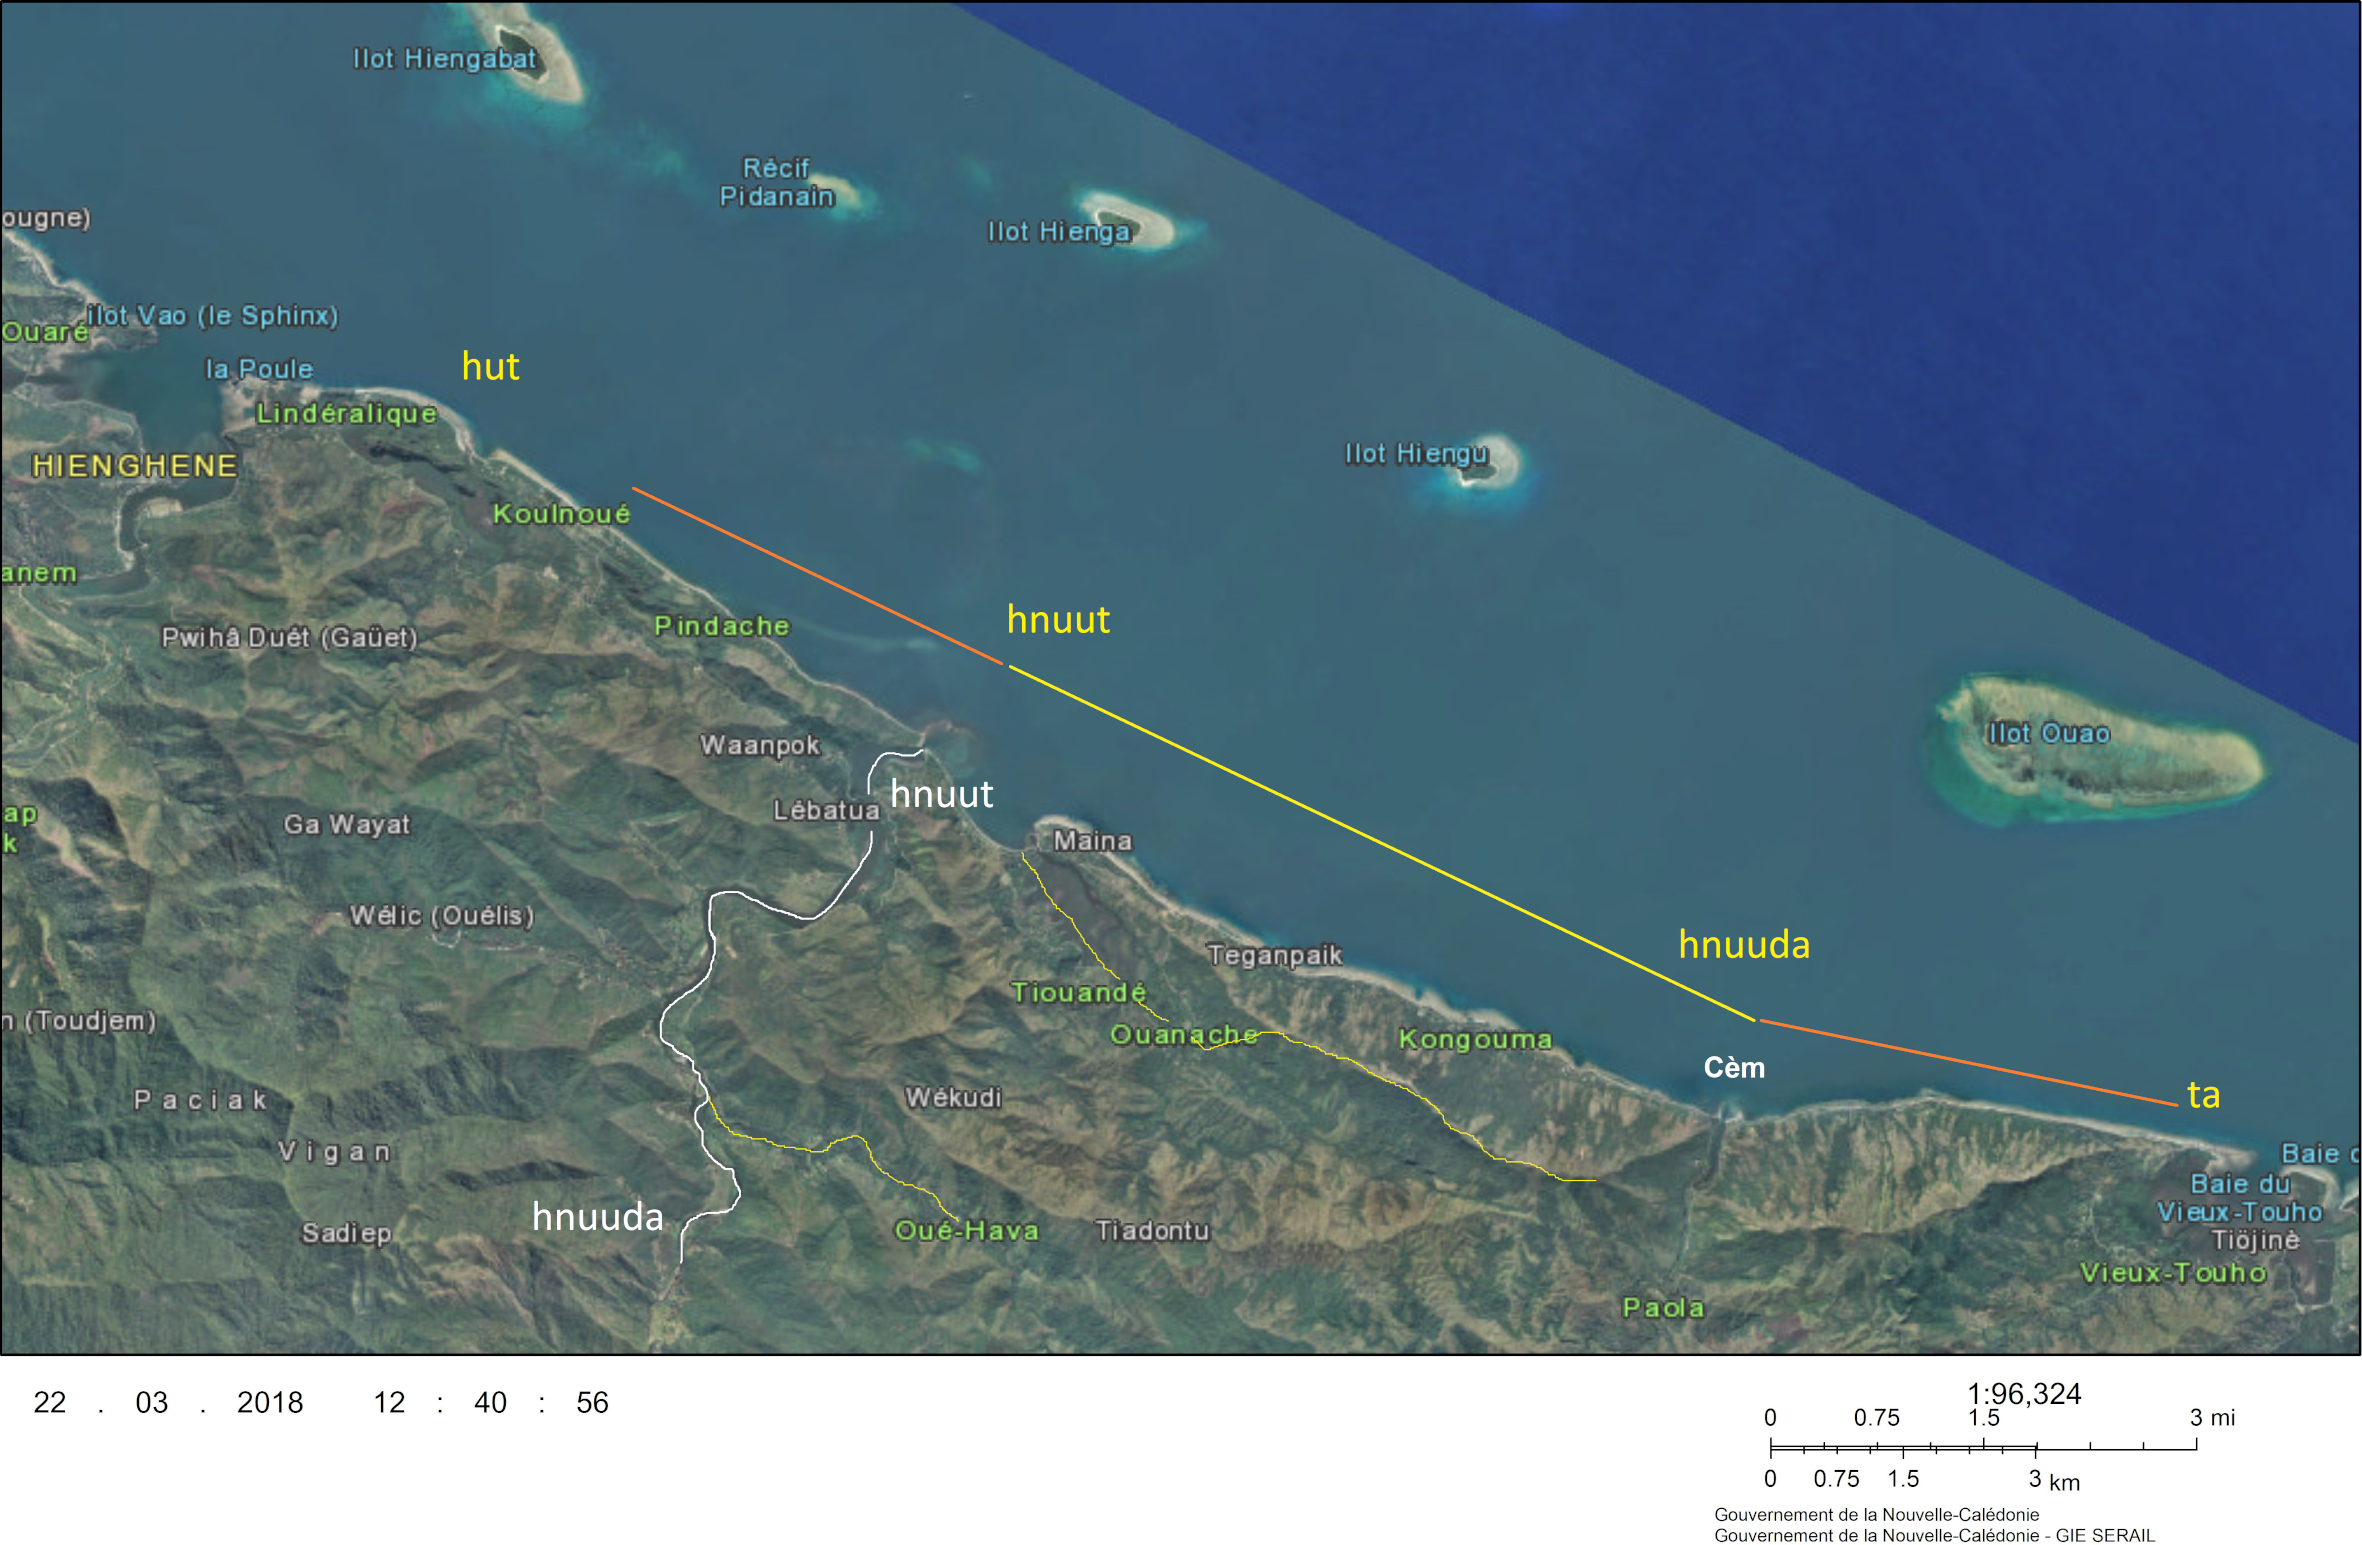
\includegraphics[width=\textwidth]{figures/map_hnuuda2.png}
	\caption{The \qu*{realm} of \textit{hnuut}. Relevant rivers marked in yellow.}
	\label{fig:map_hnuuda}
\end{figure}

\subsection{Spatial adverbs}
\label{ssec:spat_adv}
Vamale derives spatial adverbs from the verbs \textit{hut} \qu{go down}, \textit{ta} \qu{go up}, and \textit{han} \qu{move on the same level, go}. The adverbs in question, prefixed with \textit{xa-}, \textit{xa-hut} \qu{down there}, \textit{xa-da} \qu{up there}, and \textit{xa-han} \qu{over there}, form the basis of this system and are unrelated to the demonstratives in \sectref{ssec:Prox}. They are described in more detail in \sectref{ssec:prox_Adv}, but an overview is given in \Cref{tab:space}. 
Spatial words can be combined with other words (\textit{hoot xahut} \qu{far down.there}) or with each other (\textit{nyaut xahut} \qu{just down there (but too far to reach)}).

\begin{table}
	\centering
	\caption{The main motion verbs and their associated locative adverbs}
	\begin{tabular}{lll}
		\lsptoprule
		Form&Gloss&Word class\\\midrule
		\textit{cahni}& \qu{here}& adverb\\
		\textit{la}& \qu{be.here}& verb\\
		
		\textit{ta}& \qu{move up} & verb\\
		\textit{hut}& \qu{move down}& verb\\
		\textit{han}& \qu{go (same level)}& verb\\
		\textit{hnu-ut}& \qu{move downstream}&verb\\
		\textit{hnu-da}& \qu{move upstream}&verb\\
		
		\textit{xa-da}& \qu{up there}& adverb\\
		\textit{xa-hut}& \qu{down there}& adverb\\
		\textit{xa-han}& \qu{over there}& adverb\\
		\textit{xa-hnu-ut}& \qu{over there (downstream)}& adverb\\
		\textit{xa-hnu-da}& \qu{over there (upstream)}&adverb\\	
		\lspbottomrule
	\end{tabular}
	\label{tab:space}
\end{table}

 

\subsection{\textit{Nya} \qu{around, towards, inside}}
\label{ssec:nya}
\is{Space!\textit{nya} \qu{around, towards, inside}}
\textit{(H)nya} \qu{put, give, send} is a multi-purpose morpheme, especially in the context of space. One function of \textit{nya} is to combine with prepositions to form new prepositions, locating the theme as contained by or very close to the prepositioned location: \textit{ca-} \qu{at} $\rightarrow$ \textit{nye-ca-} \qu{inside} (\ref{ex:nya1}), \textit{pwa-} \qu{on top of}, $\rightarrow$ \textit{nya-pwa-} \qu{upon}, \textit{ko} \qu{on (touching a part of it)}, \textit{nya-ko} \qu{immediately on; apply on} (\ref{ex:nyako}). In this function, \textit{nya} also appears as a prefix in spatial adverbs (see \sectref{ssec:prox_Adv}), to form a proximal form (\textit{nya-ut} \qu{(put) down, down there at an arm's length}). \textit{Nya} often displays a phonologically conditioned allomorph \textit{nye} when preceding the article \textit{i} \qu{\gl{def}.\gl{sg}}, and palatal /c/, as in (\ref{ex:nya1}).


\ea\label{ex:nya1}\gll le=vwa-vaci li=apuli nye-ca i nye-ca i=mwa-n daahma\\
 3\gl{pl}=do-kernel \gl{def}.\gl{pl}=people \gl{loc}-in \gl{def}.\gl{sg} \gl{loc}-in \gl{def}.\gl{sg}=house-\gl{poss} chief\\
\glt \qu{The people were quarrelling in, in the chief's house.} {[DT:10.3]}
\z

\ea\label{ex:nyako}\gll bitake nya-ko i=yee\\
 wrap \gl{loc}-on \gl{def}.\gl{sg}=tree\\
\glt \qu{wrap around the tree} {[X9:20]}
\z

\textit{Nya} can also mean \qu{toward}, a meaning that is related to \qu{send}. In combination with spatial adverbs, \textit{nya} forms two paradigms: the series \textit{nya-xahut/nya-xada/nya-xahan} is almost equivalent in meaning to \textit{xahan} \qu{over there} etc. It means \qu{in the vicinity of X}, whereas \textit{xahan} etc. designate a more precise location.  In (\ref{ex:nya_from}) and (\ref{ex:nya_cricket}), \textit{nya} is used to express a vague area. The other paradigm combines \textit{nya-an}/\textit{nya-ut}/\textit{nya-da} \qu{send, put there/down/up} with the basic adverbial form, which yields a comparatively farther meaning, e.g. \textit{nya-an (mwa) xahan} \qu{(even) further away in this general direction} (see \sectref{ssec:spat_adv}).



\ea\label{ex:nya_from}\gll In-Fwe hapi ``In-Fwe ka e=hu-pe \textbf{nya} \textbf{nya}-da xa-da" kavi cipa a=vi i=goakan\\
 F. \gl{comp} F. \gl{cnj} 1\gl{sg}=come-\gl{dir.cp} from send-up \gl{loc}-up but \gl{neg} 3\gl{sg}=say \gl{def}.\gl{sg}=place\\
\glt \qu{Figtree-Bark said that ``[my name is] Figtree-Bark and I come from somewhere a little further up" but she didn't say the place.} {[GC:53.2]}
\z 

\ea\label{ex:nya_cricket}
\gll ka a=cuut cahni go a=cuut cai-n ka i=xa-thake i=bool. hmwakan \textbf{nya}-xahan a=cuut xahan ka i=see\\
 \gl{cnj} 3\gl{sg}=stand here \gl{cnj} 3\gl{sg}=stand behind-\gl{nspec} \gl{sbj} \gl{def}.\gl{sg}=\gl{agt}.\gl{nmlz}-throw \gl{def}.\gl{sg}=ball maybe over-there 3\gl{sg}=stand over.there \gl{sbj} \gl{def}.\gl{sg}=one\\
\glt \qu{And she stands here, and behind her stands the cricket pitcher. Maybe around there stands the other [player].} {[PJ:29]}
\z

\textit{Nya} is frequently used to locate something in a named place, especially villages, as in (\ref{ex:nya_tgnpk}). This may be a strategy to avoid having to use more specific terms such as \textit{xahut} \qu{down there}, but no clear pattern was identified.

\ea \label{ex:nya_tgnpk}\gll vwa nya theganpaik\\
 \gl{exist} around T.\\
\glt \qu{It will be in Téganpaik.} {[AG1:66]}
\z

\subsection{Same-level axis}
\is{Space!Same-level axis}
\is{Verbs!Prefixes!Manner}
Volitional displacement on the same level is expressed with the active verb \textit{han} or the derived adverb \textit{xahan} \qu{over there on the same level}. The movement of an object, e.g. in the wind, is called \textit{va(a)ya} \qu{movement, work}. Depending on the context, \textit{han} can mean \qu{go}, e.g. \textit{ha-de-ha-me} \qu{go-\gl{dir.cf}-go-\gl{dir.cp}} \qu{to and fro}, and \qu{walk}, e.g. \textit{han-maa} \qu{walk on the reef at low tide to gather sea-food}. There is an increase of the use of \textit{han} among less fluent speakers, which may be due to French influence. 

Nowadays, \textit{han} means \qu{to walk} and \textit{thêên} \qu{to run, to fly}, but the manner prefix \textit{t(h)e-} \qu{to do while walking} is probably derived from \textit{thêên}. Since this is the case for both Hienghène languages (\textit{hen} \qu{walk} in Pije, but \textit{te-} \qu{while walking}) and Voh-Koné ones, the split must be an old one.


\subsection{Centripetal/-fugal axis -\textit{me}, \textit{-le}}
\is{Space!Centripetal/-fugal}
\largerpage
There are two main suffixes used to express motion to and from the utterance's point of reference. While this center is usually the speaker, stories may set the center somewhere else more or less explicitly,\footnote{This was described for Caac as well \parencite[176]{cauchard_study_2014}.} and hypothetical or past situations can also feature these suffixes.
The movement verbs assimilate the final consonant's place of articulation to \textit{-me} \qu{\gl{dir.cp}}: \textit{ta} \qu{go up}+ \textit{-me} $\rightarrow$ \textit{tame} \qu{come up}, \textit{hut} \qu{go down} + \textit{-me} $\rightarrow$ \textit{hupe} \qu{come down}, \textit{han} \qu{go} + \textit{-me} $\rightarrow$ \textit{hame} \qu{come}. The other suffix \textit{-le} \qu{\gl{dir.cf}} assimilates to the verb's final consonant: \textit{ta-le} \qu{leave upwards}, \textit{hut-e} \qu{leave downwards}, and \textit{han-de} \qu{go away}. The latter is another example of the relationship between alveolar plosives and liquids mentioned in \sectref{ssec:ka_CL}.

Motion verbs can be added to a verb phrase if a centripetal or centrifugal meaning is needed, as other verbs cannot take \textit{-me} or \textit{-le}, as in (\ref{ex:added_hame}).
\ea \label{ex:added_hame}\gll kona sili sahmwa ha-me sili sahmwa ha-me\\ then pierce other.way go-\gl{dir.cp} pierce other.way go-\gl{dir.cp}\\
\glt \qu{Then he backs [the truck] up, backs it up.} {[KG:466]}
\z


\subsection{Origin of motion}
\label{ssec:mo_ko}
\is{Space!Origin of motion \textit{moo}}
In order to express the origin of a motion, \textit{moo} \qu{stay} is preposed to the source, and postposed to the motion verb, as in (\ref{ex:Vmoo}).

\ea \label{ex:Vmoo}\gll na tha go=saat moo cahni\\
 \gl{dem} \gl{ass} 2\gl{sg}=wade from here \\
\glt \qu{You wade in the water from here.} {[RP:6]}
\z

\subsection{Others}

This section has not made a complete description of spatial expressions in Vamale, a daunting task that has become a PhD thesis in its own right for both Nengone \parencite{bearune_lexpression_2012} and Caac \parencite{cauchard_study_2014}. The chapter mostly focused on the main axes of motion, proximity,\footnote{Proximal and distal demonstratives are discussed in \sectref{ssec:Prox}.} and centripetal/centrifugal motion, but there is a lexical field of prepositions (e.g. \textit{pwa-} \qu{on}, \textit{xala-} \qu{under}, \textit{cela-} \qu{beside}, \textit{patemwano} \qu{right next to}, \textit{ca-} \qu{at}) (see \sectref{ssec:WCPrepoNouns}), manner verbs (e.g. \textit{falogavi} \qu{move across diagonally}), and verbs describing motion more specifically, e.g. \textit{cop} \qu{go over a mountain, go to the other coast; surpass someone} or \textit{saat}\footnote{There are also \textit{sesaat} \qu{walk slowly, sneak}, and \textit{sesaaleke} \qu{stalk} which could be related.} \qu{walk through water, ford a river}. The next section leaves the lexical domain of space and addresses productive prefixes denoting posture and ways of doing things.

\section{Prefixes}
\label{sec:VPrefix}
\is{Verbs!Prefixes}
\largerpage
The following derivational prefixes are distinct from TAM markers in that they are not independent words, although they express similar meanings, and are partly sensitive to aktionsart. \Cref{tab:pref_Manner} lists them with examples.
%Many of the prefixes are derived from verbs. %todo bar
Prefixes of manner are all derived from verbs and in many cases lexicalized, though some still appear productive. \textit{The-} is a polysemous prefix, as it not only contributes its expected \qu{do while walking/running} meaning to verbs, but also takes more aspectual meanings, depending on the verb and its context (see \sectref{ssec:the}). Prefixes are presented here in \Cref{ChapterVerbs} while aspectual markers, which are own words, are described in  \Cref{ChapterAspect}, and anything that is exclusive to the verb phrase but not part of the verb, in \chapref{ChapterVP}.

\subsection{Prefixes of manner}
\label{sec:Manner}
\is{Verbs!Prefixes!Manner}
Manner prefixes can be added to roots to express how something is done, and have in many cases become lexicalized, i.e. are not added to new words, but can be identified as bearing meaning in several verbs. % %todo what is a lexicalized environment?
For example, \citeauthor{rivierre_bwatoo_2006} analyze some words as complex (e.g. \textit{tha-bilo-ke} \qu{to kill}, \citeyear[61]{rivierre_bwatoo_2006}), which are not attested without their manner prefix, or indeed with another prefix, in Vamale. Bound verbal forms which are still attested in the dictionary include: 
\begin{enumerate}
	\item \textit{-bii} \qu{crack} from POc *piti(k) \qu{crack} \parencite[276]{ross_lexicon_1998},\begin{enumerate}
		\item  \textit{cu-bi(i)} \qu{break bread} 
		\item \textit{cu-bite} \qu{be squashed by a crowd}
		\item \textit{caa-bite} \qu{harvest}
		\item \textit{ca-bi} \qu{smash something brittle by hand or blunt tool}
	\end{enumerate}
	\item \textit{-bwane} \qu{split} from POc *pʷalaq \qu{split} \parencite[265]{ross_lexicon_1998}, e.g. \textit{tha-bwane vai} \qu{split stone}, \qu{Téganpaïk (a village name)}
	\item \textit{-bali} \qu{drive in}, e.g. \textit{tha-bali} \qu{to nail}, \textit{coo-bahli} \qu{push someone away with the hand}
	\item \textit{-theeke} \qu{push}
	\begin{enumerate}
	\item \textit{pitheeke} \qu{to push someone away}
	\item \textit{caatheeke} \qu{push away with a stick}
	\item \textit{sibatheeke} \qu{push someone in a direction}
	\item \textit{tha-theeke} \qu{kill with a spear}
	\item possibly \textit{theeke} \qu{blow on food}
	\end{enumerate}
Note that in the first three examples listed for \textit{-theeke}, the preceding parts are transparent.
\end{enumerate} Manner prefixes have been described in \citetitle{ozanne-rivierre_verbal_2004}, called ``classificatory prefixes" there \parencite[349]{ozanne-rivierre_verbal_2004}, and are typical of New Caledonian languages, albeit more frequent in Southern languages than in Northern ones. It is possible that a compound consisting of a shortened transitive manner verb and an action verb was already a feature of Proto-Mainland \parencite[354]{ozanne-rivierre_verbal_2004}, as these prefixes appear throughout the main island, but have diversified clearly within the two groups North and South. Having a variety of verbs for striking with different tools is an old feature of Oceanic. \Cref{tab:POcV} (page~\pageref{tab:POcV}) gives a short selection of Proto-Oceanic verbs.\footnote{The form *sasa is given by \parencite{grace_proto-oceanic_1969}.} The posture prefixes \textit{cu-} \qu{do standing}, \textit{ta-} \qu{do sitting}, see (\ref{ex:ta-meebam}), and \textit{mi-} \qu{do lying down}, are unique to Northern languages \parencite[356]{ozanne-rivierre_verbal_2004}. Note that Ozanne-Rivierre and Rivierre call verbs prefixed by the morphemes described here ``compound verbs", whereas I use the term exclusively for verbs where all components are also attested as single head verbs.

%\textit{tha-} *sasa \qu{hunt, thrash, a whip} grace 1969xx, \textit{co-} PEO *taus(i) \qu{pluck} \parencite[279]{ross_lexicon_1998}
\begin{table}[p]
	\caption{Proto-Oceanic verbs for hitting \parencite[267]{ross_lexicon_1998}}
	\begin{tabularx}{\textwidth}{lQ}
	\lsptoprule
		 POc & Meaning\\\midrule
		 *sasa &\qu{hunt, thrash, a whip}\\
		  *punu(q), *punuq-i-& \qu{hit, strike, fight, kill}\\
		  *qubu, *qubWi-& \qu{hit with fist or with a weapon}\\
		  *rapu(t), *raput-i- & \qu{hit with hand or stick, slash}\\
		  *tutuk, *tuki[-]& \qu{pound, mash by pounding, hammer, crack by hammering}\\
		  *putu(k) and *butu(k), *butuk-i-& \qu{repeatedly knock,  pound, beat}\\
		  *qatu(1), *qatu-J-i- & \qu{strike from above, pound}\\
		  *babak, *baki[-]  & \qu{strike one against another, knock}\\
		  *tupu, *tupu-i-& \qu{knock against, knock over, stub (toe), stumble against}\\
		  *pwasa(r,R), *pwasa(r,R)-i­& \qu{slap, hit}\\
	  \lspbottomrule
	\end{tabularx}
\label{tab:POcV}
\end{table}
 
\begin{table}[p]
	\caption{Manner prefixes, their likely origins, with examples.}
	\small
	\fittable{%
	\begin{tabular}{lllll}
		\lsptoprule
		Form & Meaning & Origin & Example & Meaning\\
		\midrule
		\textit{ca-} & hit with hand & & \textit{cabi} & \qu{smash something brittle}\\
		\textit{caa-}& set down foot& \textit{caa}&\textit{caa-gati} & \qu{crush something soft}  \\
		&&&\textit{caa-thiho} & \qu{limp}\\
		\textit{co}- & with hand & &\textit{co-gavi} &\qu{break by pulling} \\
		&&&	\textit{co-bahli}&\qu{push off by hand}\\
		\textit{ta}- & sitting & \textit{tabo} & \textit{ta-meebam} & \qu{sit-sleep; sleep in a sitting position}\\
		\textit{cu-} & standing & \textit{cuut}& \textit{cu-vathan-ke} & \qu{stand-each-\gl{tr}; stand apart from e. o.}\\
		\textit{mi-} & lying & \textit{majit}&  \textit{mi-xaleke} & \qu{lay-see; have a vision}\\
		\textit{tha-} & forcefully & \textit{thake} & \textit{tha-biloke} & \qu{strongly-kill; kill with a strike}\\
		&&&\textit{tha-gavi}&\qu{strongly-cut; cut with one strike}\\
		\textit{so-} & touch & \textit{soot} & \textit{so-teet} & \qu{touch-lazy; do carelessly}\\
		\textit{fa-}%\footnotemark
		& speak& \textit{fati} & \textit{fa-xhopwen} & \qu{talk big, boast}\\
		\textit{t(h)e-} & do walking & \textit{thêên} & \textit{t(h)e-thagavi} &\qu{walk-cut; take a short-cut}\\ 
		\lspbottomrule
	\end{tabular}}
\label{tab:pref_Manner}
\end{table}
%\footnotetext{\textit{fa-vamale} \qu{speak Vamale} seems to be a de-nominal derivation, whereas the other prefixes attach onto verbs.}

\ea \label{ex:ta-meebam}
\gll bo tha xa-vaaya-n-eo i=  m=e=ta-meebam aa ca-n sohmun\\
 \gl{irr} \gl{ass} \gl{agt}.\gl{nmlz}-work-\gl{poss}-1\gl{sg}.\gl{poss} \gl{def}.\gl{sg} \gl{subr}=1\gl{sg}=sit-sleep uuh in-\gl{nspec} study\\
\glt \qu{That would be my habit, the\ldots if I slept sitting in school.} {[2017-10-30 Pauty Ecole et punition:10]}
\z

\subsection{\textit{the-} }
\label{ssec:the}
\is{Verbs!Prefixes!\textit{the-} \qu{quickly, a bit; while walking}}
The prefix \textit{the-} is halfway between a prefix of manner and an aspect marker. It likely comes from \textit{thêên} \qu{run, fly} and still exists as a manner prefix, as illustrated in the words \textit{the-thagavi} \qu{take a shortcut} and \textit{the-yathô} \qu{walk-stress; walk in a hurry}. It seems, however, that this use has become lexicalized.
%\ex
%\label{ex:the_manner}
%
%\ili{}{}{} Jean-Philippe, 11.7.2019, p.20
%\gll the-th
%
%
%
%\glt
%
%
%\z

The productive, non-manner prefix \textit{t(h)e-} has two meanings, depending on the aktionsart of the verb. With punctual verbs, it means \qu{do quickly, a bit}. With durative ones, it means \qu{do continually since earlier}, often with reference to another event, e.g. \textit{the-xaleke} \qu{look at constantly}, and (\ref{ex:constant_the}). This is likely due to its putative origin \textit{thêên} \qu{run, fly}. In imperatives, \textit{the-} always asks for immediate action: \qu{do this now}. 
While \textit{the-}prefixed verbs, when preceded by TAM markers, often do not take on idiosyncratic meanings, some combinations are interesting. Frequentative \textit{mu}, habitual \textit{xa}, and imperfective/future \textit{bwa} do not change the meaning, but \textit{pa} \qu{\gl{prf}} excludes an interpretation of the event as quickly done; the yielded meaning focuses on the time spent on it (``it took me a long time to do it"). This effect is even stronger with \textit{pa ja} \qu{\gl{prf}.\gl{prf}}. With progressive \textit{kon}, \textit{the-} means \qu{right now, immediately}. 
With durative verbs, \textit{the-} takes on a durative, imperfective meaning, and is similar in function to the adverb \textit{hnyana} \qu{constantly}.\footnote{See \textit{hnyana-} \qu{breath}, from which it is probably derived.} Compare the pair of examples (\ref{ex:constant_hnyana}) and (\ref{ex:constant_the}) for said similar meanings, but see examples (\ref{ex:the_vs_hnyana}) and (\ref{ex:the_vs_hnyana2}) for the differences.


\ea\label{ex:constant_hnyana} \gll ceme o vaya tha xalo ko-n tele hnyana\\
 \gl{subr}.1\gl{sg} \gl{irr} work \gl{ass} gaze \gl{obl}-\gl{nspec} TV constantly\\
\glt \qu{Whenever/If ever I work, he'll watch TV (while and as long as I work). [Jean-Philippe, 11.7.2019, p.20]} {}
\z 

\ea\label{ex:constant_the}
\gll ceme o vaya tha the-xalo kon tele\\
 \gl{subr}.1\gl{sg} \gl{irr} work \gl{ass} \gl{thedur}-gaze \gl{obl}-\gl{nspec} TV\\
\glt \qu{Whenever/If ever I work, he'll watch TV (while and as long as I work).}
\z

\begin{sloppypar}
When describing a situation that is unique and limited in time, \textit{the-} and \textit{hnyana} are interchangeable. However, more general, or abstract, situations, \textit{the-} \qu{\gl{thedur}} takes a meaning similar to \textit{the-} \qu{\textsc{the\textsubscript{punct}}}, see examples (\ref{ex:the_vs_hnyana}) and (\ref{ex:the_vs_hnyana2}). This is reminiscent of \textit{mwa} \qu{again, now, however} in \sectref{sec:WCRepetitive}.
\end{sloppypar}

	\ea \label{ex:the_vs_hnyana}
	\gll tha go=the-xaleke\\
		 \gl{ass} 2\gl{sg}=\gl{thedur}-see\\
	\glt \qu{You see now.}
	\z 
		
	\ea \label{ex:the_vs_hnyana2}
		\gll tha go=xaleke hnyana\\
	 \gl{ass} 2\gl{sg}=see constantly\\
	\glt \qu{You often see.}
		\z


%\subction{Imperative use of \textit{the-}, and \textit{xhaa-}}
\is{Clauses!Imperative clauses}

\textit{The-} can be used with imperative verbs, where it asks for immediate action: \qu{do this now, do this quickly}. Another prefix, \textit{xhaa-} \qu{\gl{att}}, only appears in the imperative mood and acts as an attenuative prefix, \qu{do a bit} (\ref{ex:the_imp}). In some scenarios, the two have similar meanings.% shortens vowel if combined with e.g. \textit{da}, \textit{the}, etc. possibly not phonemically long vowel.

\ea \label{ex:the_imp}\gll xhaa-thagavi ye-mwago ma go=xaleke i=vaaya koo-n\\
 \gl{att}-cut tree-mango \gl{subr} 2\gl{sg}=see \gl{def}.\gl{sg}=work \gl{obl}-\gl{nspec}\\
\glt \qu{Just (try to) cut a mango tree and you’ll see the work it is.} {[example sentence provided for the dictionary entry on \textit{xhaa}]}
\z
 
The attenuative meaning of \textit{xhaa-} is found with imperative \textit{the-} when the latter is used to suggest that the action asked for will be quick. The difference, however, is that \textit{the}- suggests a quickly done task, whereas \textit{xhaa}- means you do something for a short while, without necessarily finishing what you started. \textit{The-} and \textit{xha(a)-} can be combined (\ref{ex:xhaa}). When combined, their meaning depends on the verb's aktionsart: \qu{quickly do now (\gl{punc})}, \qu{do a non-committally big or small bit of it (\gl{dur})}.

\ea \label{ex:xhaa}
\gll xhaa-the-thagavi cahni\\
 \gl{att}-\textsc{the\textsubscript{punct}}-cut here\\
\glt \qu{Just cut it here real quick.}
\z

\subsection{\textit{da} \qu{do first}, \textit{ra-} \qu{do afterwards}}
\is{Verbs!Prefixes!\textit{da} \qu{do first}}
Two morphemes can be used to sort an action with respect to other actions: \textit{da(a)} \qu{do first} (\ref{ex:da_first}), and \textit{ra-} \qu{do afterwards} (\ref{ex:ra}). Note that the latter is the only phonemic example of /ɾ/, and was only encountered in elicitation sessions. A similar \textit{ra-} \qu{continue to (while others have stopped)} in Bwatoo is perhaps cognate \parencite[56]{rivierre_bwatoo_2006}.


\ea\label{ex:da_first}\gll da bale ca i=xhoogo-n-go, ka go=bo vwa thuan nya pala li=been\\
 do.first broom in \gl{def}.\gl{sg}=home-\gl{poss}-2\gl{sg}.\gl{poss} \gl{cnj} 2\gl{sg}=\gl{irr} do do.well in home \gl{def}.\gl{pl}=peer\\
\glt \qu{First clean up your home, then you (may) go clean up other homes.} {[Proverb]}
\z 


\ea\label{ex:ra}\gll go=bo ra-ha-me\\
 2\gl{sg}=\gl{irr} later-go-\gl{dir.cp}\\
\glt \qu{You'll come afterwards.} {[21.07.2019 p.42]}
\z
%Suffix "do in advance, go ahead"

\textit{da} \qu{to do first, in advance} is more common than \textit{ra-}, and contrary to the latter, can take stress (\ref{ex:da1}). It does not head phrases, however. It will hence be analyzed as a pre-verb.


\ea\label{ex:da1}
[e ˈⁿdaː viː ɲãkɔ̃ːm]\\
\gll e=da vii nyakoo-m\\
 1\gl{sg}=in.advance tell \gl{obl}-2\gl{sg}\\
\glt \qu{I am warning you.} {[D3:79]}
\z


\ea
\gll  gase=da xhwi-aman kon gase=bwa vwa \textit{coutume}\\
 1\gl{pl}.\gl{incl}=in.advance eat-thing then 1\gl{pl}.\gl{incl}=\gl{ipfv} do custom\\
\glt \qu{We'll eat first, then we'll conduct the ceremony.} {[L1:31]}
\z

%\ea
%\ea
%
%\gll han-da
% go-ahead
%\glt \qu{go ahead}
%
%\ea
%
%\gll vwa-ta 
% do-advance
%\glt \qu{do in advance}
%
%\z

\subsection{Pluractional \textit{e-}}
\label{ssec:pluriactional}
\is{Pluractional \textit{e-}}
\is{Verbs!Prefixes!Pluri-actional}
A pluractional prefix \textit{e-} occurs in various constructions where several entities perform the same action at the same time, but not to each other, e.g. (\ref{ex:ehan_caile}) and (\ref{ex:etipwa}). The prefix is reconstructed to be a reflex of POc *paRi-, which otherwise has reflexive, reciprocal, and middle functions. If \textit{e-} were left out, the pluractional meaning would be lost, and the participants would be engaged in their activities in a more individual manner: compare examples (\ref{ex:ehan_cain}) and (\ref{ex:ehan_caile}) to \textit{le han cai-n} \qu{They follow him} and \textit{le han cai-le} \qu{They follow them}. Note that in constructions such as (\ref{ex:ehan_caile}), the meaning is somewhat in between reciprocal (they follow each other), further described in \sectref{sec:refl}, and pluractional (they each follow a different person). This is called ``chaining" by Bril, and widely attested throughout the archipelago \parencite[32, 47]{bril_semantic_2005b}.
%Why is this MID? Can the same predicate occur without e-? Or is it a medium tantum? Or is it just the plurality of referents that triggers/favors (?) the MID marking?

\ea\label{ex:ehan_cain}\gll le=e-han cai-n\\
 3\gl{pl}=\gl{mid}-go behind-3\gl{sg}\\
\glt \qu{They \textit{all} follow him/her.} {[07.11.18 p.93]}
\z


\ea\label{ex:ehan_caile}
%This is not really reciprocal is it? It seems more like a "all do this"\gll le=e-han cai-le\\
 3\gl{pl}=\gl{mid}-go behind-3\gl{pl}\\
\glt \qu{They walk one after the other (single file).} {[07.11.18 p.93]}
\z


\ea\label{ex:etipwa}\gll le=e-tipwa pu ka li=xhaapwe sep\\
 3\gl{pl}=\gl{mid}-fall be.on.the.ground \gl{sbj} \gl{def}.\gl{pl}=fruit coco\\
\glt \qu{The coconuts fell all together.}\\\relax
[vamale-181107-jpnelemwa-04: 00:01:19-00:01:24]
\z
 

\ea\label{ex:tipwa_hato}\gll le=tipwa hut hato ka li=xhaapwe sep\\
 3\gl{pl}=fall go.down do.alone \gl{sbj} \gl{def}.\gl{pl}=fruit coco\\
\glt \qu{The coconuts fell by themselves (without known cause).} {[vamale-181107.jpnelemwa-04: 00:00:30- 00:00:32]}
\z

A difference between reference and occurrence, i.e. whether several things happen at once, or the same action several times, is made analytically, by adding \textit{sisipo} \qu{together} at the end of the verb phrase, or \textit{vataan} \qu{each, individually} as a preverb. 

In (\ref{ex:ve-moo}), similarly to contexts of \textit{mee} \qu{all} described in \sectref{ssec:se-me}, the action is performed by several people together. However, while \textit{mee} usually merely implies that out of a group, everyone participates, \textit{(v)e-} here adds a semantic trait of indistinguishability \parencite[66--73]{kemmer_middle_1993}. The participants sit together and form an indistinct group, whose members do not participate in the sitting separately.

%\todo{How can the agents be affected by staying and going down? You would have to show a contrast and actually test for affectedness...}
%xx

\ea \label{ex:ve-moo}
%\ili{}{}{} 
\gll go tha le=ve-moo mwa moo mwa \\
 well \gl{ass} 3\gl{pl}=\gl{mid}-stay \gl{rep} stay \gl{rep}\\
\glt \qu{Well and then they all stay together, stay.} {[KL:220]}
\z


\ea
%\ili{}{}{
\gll th=abe xa-e-hut ca-n jigo\\
 \gl{ass}=1\gl{pl}.\gl{excl} \gl{nmlz}.\gl{agt}-\gl{mid}-go.down in-\gl{nspec} mangrove\\
\glt \qu{We all used to go down to the mangrove (to play).} {[PE1:107 ]}
\z


\section{Complex verbs}
\label{sec:ComplexV}
\is{Verbs!Complex verbs}
This section introduces three ways in which Vamale forms complex verbs. Following an ancient Oceanic tradition, some verbs are reduplicated. Though not very prevalent in Vamale, some examples are discussed in \sectref{sec:redup}. Verbs and other verbs may join to form compounds, and verbs and nouns are also frequent partners in the creation of new words. 

\subsection{Reduplication}
\label{sec:redup}
\is{Reduplication}
\is{Verbs!Reduplication}
True reduplication in Vamale is rare. Cases abound where a verb is repeated, to express the length, urgency, intensity etc. of a notion: most frequent is the context of a serial verb construction (described in \sectref{sec:SVC}), but verbs are also repeated in a poetic context such as in (\ref{ex:xho}), or in a playful one (\ref{ex:javelo}). These verbs usually have their own prosodic environment and the whole construction is lexically transparent.\largerpage[-1]


\ea \label{ex:xho}
(Cicada-hunting children's song)\\
\gll tabo tabo li=xho thamo thêên thêên li=xho xayu\\
 sit sit \gl{def}.\gl{pl}=cicada female fly fly \gl{def}.\gl{pl}=cicada male\\
\glt \qu{Sit sit oh female cicadas [full of eggs], fly fly (away) oh male cicadas.} {[vamale-181121-xho\_thamo]}
\z

\ea \label{ex:javelo}
(Stone-skipping call)\\
\gll jaaaavelo-velo-velo-velo\\
 ricochet\\
\glt \qu{ricochet-chet-chet-chet}
\z

The attested cases in which a word is repeated and forms a new word are the following: \textit{fwa-fwa} \qu{hole-hole} \qu{full of holes}, \textit{vaya-vaya} \qu{move-move} \qu{wobbly}, and \textit{xhasaat-xhasaat} \qu{jump-jump} \qu{hobble, jump around on one foot or to get warm}. While the consultant said that there were many other cases, I found none.

\subsection{Compound verbs}
\label{ssec:CompoundV}
\is{Verbs!Compound verbs}
\largerpage[-2]
Compound verbs are composed of a verb, which determines the resulting construction's word-class and often plays a dominant role in its semantics, and another element. The interesting case of the verb \textit{hnya} \qu{put, send} and spatial adverbs such as \textit{xahan} \qu{over there}, which combine to \textit{(h)nya-xahan} \qu{in this direction}, is an exception. These combined words are adverbs (see \sectref{ssec:nya}), as evidenced by verb phrases like \textit{hnya hnya-xada} \qu{put over there}, and will not be discussed further here.

An important group of compound verbs are composed of the vague verb \textit{vwa} \qu{do}, and a specifying verb, e.g. \textit{vwa-suu} \qu{do break} \qu{pay someone}, \textit{vwa tau} \qu{do impact} \qu{fish},\footnote{This is almost certainly a taboo avoidance strategy. Hunters never use \textit{vap} \qu{to hunt} if they go out, instead they say \textit{balan thaap} \qu{length nyaouli [a savannah tree species]} when describing their plans, to avoid bad luck. \textit{Vwa tau} would have replaced the marked word. Word avoidance taboos are commonplace in this region of the world. Perhaps the word for \qu{wound}, \textit{ape aman} \qu{trace\slash track of something} is kept vague on purpose.\is{Word avoidance taboo}} or \textit{vwa-thiho} \qu{do-stumble} \qu{do by accident}. Another group, small but very often used, are the lexicalized serial verb constructions (SVCs) with \textit{fe} \qu{take} and motion verbs, e.g. (\ref{ex:feame}). Other verb compounds also seem to be lexicalized SVCs, e.g. \textit{saahma-cuut} \qu{rise-be.standing} \qu{to stand up}, and \textit{ha-de-ha-me} \qu{go-\gl{dir.cf}-go-\gl{dir.cp}} \qu{move to and fro}.

\ea \label{ex:feame}
\gll fe-(h)a(n)-me\\
 take-go-\gl{dir.cp}\\
\glt \qu{bring}
\z 

\subsection{Incorporated object constructions}
\label{ssec:CompV}
\is{Verbs!Incorporated object construction}
\begin{sloppypar}
On top of combining verbs with other verbs, Vamale also forms grammatical words from verbs and non-specific arguments: this includes everyday activities incorporating the most common undergoer, e.g. \textit{xhajake-lait} \qu{eat.starchy-rice} \qu{eat rice}, \textit{xhwi-aman} \qu{eat.proteiny-something} \qu{eat something}, \textit{vai-xam} \qu{weave mats}. This is called ``incorporated object construction" by \citet[357]{ozanne-rivierre_verbal_2004}. There are numerous verbs formed with \textit{vwa} \qu{do}, e.g. \textit{vwa-vaci} \qu{do-pit, hard part}  \qu{to argue}, \textit{vwa-ikin} \qu{do-meaty.side-dish} \qu{to eat tubers with meat}, \textit{vwa-khêt} \qu{do-quarz, blade} \qu{to shave}. All the verbs mentioned form a single stress-contour and cannot be split without losing their overall meaning.
Some nominalized forms can contain complex verbs including a noun, such as \textit{xa-thêên-fe-\textbf{fati}} \qu{\gl{agt}.\gl{nmlz}-run-take-word} \qu{messenger} and \textit{xa-fe-ta-me-\textbf{mapeke}} \qu{\gl{agt}.\gl{nmlz}-take-go.up-\gl{dir.cp}-bright} \qu{morning star}. 
\end{sloppypar}

\section{Nominal derivation}
\label{sec:NomDeriv}
\is{Verbs!Nominalization}
\is{Nominalization}

Vamale derives nouns from verbs either by using nominalizing prefixes or simply by stripping the verb from its subject indices (be they proclitics or suffixes), and preposing an article. The nominalizers (e.g. \textit{e-, xa, hun-}) are analyzed here as prefixes because they directly attach to the root, the article, e.g. \textit{i=} \qu{\gl{def}.\gl{sg}} can only occur before it (\textit{i=xa-xaleke, *xa=i=xaleke}). 
%``Derivation" means that one only needs a subject marker on the stem to make it a verb, but you don't, instead you put a nominalizer, and you have a noun.xx
The resulting nominalized construction can be used as an argument with a verb or a preposition and can be possessed by another nominal phrase. The possessor is not, however, understood to be the agent of the action, as in English (e.g. \qu{my seeing the brother}), except for intransitive verbs. Instead, the possessor denotes the undergoer. %%todo sondern wie wird es verstanden, oder wo sagst du mehr darüber?
%What makes them nominal is the slot. \textit{i=} can attach to it, adjectives can, it can function as an argument to a verb (whereas a verb cannot have a verb as an argument I think).xx
Whether a given verb is nominalized via prefixation or stripping is lexically determined, since nominalizing via stripping is not accepted for some verbs (e.g. \textit{*i thapoke} \qu{the beginning}, or \textit{*i hmanan} \qu{his/her hunger}). Another example is \textit{hun-vwa kan} \qu{manner-do it; the style of doing it, the act of doing it} which cannot be \textit{*vwa kan} or even \textit{*vwa}. Both stripped and prefixed nominalizations may include arguments, as in (\ref{ex:i_jili}), but not TAM markers. 
Stripped nominalizations, contrary to the other de-verbal constructions detailed below, do not express a subject through possessive means, but keep the same strategy as normal verb phrases, i.e. using a noun phrase flagged with \textit{ka} \qu{sbj}: \textit{ka li=apuli} \qu{\gl{sbj} \gl{def}.\gl{pl}=person} in (\ref{ex:i_jili}). There are two relatively neutral prefixes, \textit{ape-X} meaning \qu{fact of doing X}, and \textit{hun-} \qu{manner of doing X}, though \textit{hun-} was the only one readily used by speakers for novel constructions. 

%
%\begin{enumerate}
%	\item We have \textbf{canonical nouns}, alienably or inalienably possessed.They alone do not constitute a clause. (*\textit{i daahma.}).
%	\begin{enumerate}
%		\item We have verbs that are nominalized with an obligatory  \textsc{nmlz} prefix when preceded by an article: \textit{i ape-hnyimake-aman} \qu{the fact-think-something; the thought} %(tentatively called "the NOM-needers").
%		\begin{itemize}
%			\item \textit{thapoke} \qu{begin}, ambitransitive, must be \textit{ape-thapoke-ka-n} (place-begin-acc-inan) \qu{the moment of beginning} or \textit{hun-thapoke-o/go/a/...} (manner-begin-1\gl{sg}...) \qu{the a{}ct of beginning} (this pattern is the same for all similarly nominalized verbs).
%			\item \textit{vii} \qu{say}, transitive, must carry the prefix \textit{hun-}.
%			\item \textit{moo} \qu{stay} \textbf{intransitive} must be \textit{hun-moo}.
%		\end{itemize}
%		\item We have nominalizations of entire verb phrases. This is still productive and probably an old construction.  like \textit{jili} \qu{build with wood}. They keep their object NPs in the VP. %No possession of objects like in English \textit{the speaking \textbf{of} the word}. 
%		No possession of the resulting construction attested. What works is a complete clause with a \textit{ka} subject nominalized with an article, as shown in \ref{ex:i_jili}. 
%	\end{enumerate}
%\end{enumerate}  

	\ea
	\label{ex:i_jili}
	\gll e=xaleke i=jili i=bwaakala ka li=apuli\textsubscript{\gl{sbj}}\\
	 1\gl{sg}=see \gl{art}.\gl{sg}=build.with.wood \gl{art}.\gl{sg}=pirogue \gl{sbj} \gl{art}.\gl{pl}=people\\	
	\glt \qu{I see the building of the pirogue by the men.}
		\z



\subsection{\textit{e}-}
\label{ssec:ins.nmlz}
\is{Nominalization!Instrumental nominalizer}
The instrumental nominalizer \textit{e-} has \textit{fe-} and \textit{ve-} cognates in related Northern languages. It is likely that \textit{v-} was only recently dropped, as the word for \qu{spoon} was only coined in the last 150 years, and is \textit{vetupi} from \textit{tuuvi} \qu{scoop up from liquid} (though a loan from a more archaic dialect is not excluded). The word for \qu{learning} \textit{eca} is still listed as \textit{veca} by Leenhardt (1946) and pronounced that way by Chief Luc. In Nelêmwa, a similar morpheme \textit{-ve-} or \textit{-vi-} depending on animacy \parencite[194]{bril_complex_2004}, comes from \textit{fhe} \qu{take} in Nêlêmwa (\textit{fe} in Vamale), though it is not a nominalizer (\textit{baa-}, \citealt[74]{bril_nelemwa_2002}). Our nominalizer \textit{e-} might have a similar background to Nelêmwa \textit{-ve-}, being derived from \textit{fe} \qu{to take}. Cèmuhî and Paicî use \textit{be-} \qu{\gl{ins}.\gl{nmlz}} \parencites[257]{rivierre_langue_1980}[42]{rivierre_dictionnaire_1983}, versus the reciprocal/middle \textit{pi-} \parencites[257]{rivierre_langue_1980}[363]{rivierre_dictionnaire_1983}.

\begin{enumerate}
	\item \textit{e-vwa-tiike} \qu{pen} (lit. \qu{\gl{ins}.\gl{nmlz}-make-write})
	\item \textit{e-xadae-ke} \qu{blessing} (lit. \qu{\gl{ins}.\gl{nmlz}-up.there-\gl{tr}})
	\item \textit{e-vwadi-ya-n} \qu{thumb} (lit. \qu{\gl{ins}.\gl{nmlz}-peel-starchy.food-3\gl{sg}.\gl{poss}})
	\item \textit{e-xhwali-aman} \qu{fork} (lit. \qu{\gl{ins}.\gl{nmlz}-stab-thing})
	\item \textit{e-ja} \qu{scales} (lit. \qu{\gl{ins}.\gl{nmlz}-measure, weigh})
\end{enumerate}

Other items look like nominalizations, but the meaning of the presumed base form is lost: \textit{e-xhaat} \qu{paddle}, \textit{e-thadala} \qu{fruit-picking rod}. 

\subsection{\textit{xa}-}
\label{ssec:agt.nmlz}
\is{Nominalization!Agentive nominalizer}
\textit{Xa-} \qu{\gl{agt}.\gl{nmlz}}, an agentive nominalizer, is probably derived from \textit{xayu} \qu{male}. Since in Vamale, modifiers usually follow the modified, and possessors the possessum, \textit{xa-} may be an old phrase head, now incorporated into the former modifying phrase. The nominalizer may have developed from a noun phrase with an optionally marked relative clause (\ref{ex:xavwatau}), which was gradually reduced to \textit{xay(u) vwa-tau}, and finally to \textit{xa-vwa-tau} \qu{fisherman}.

	\ea \label{ex:xavwatau}
		\gll xayu (a=a=) vwa-tau\\
	 male (\gl{rel}=3\gl{sg}) make-impact\\
	\glt \qu{the man who fishes} (the relativizer \textit{a} is often omitted)
		\z

The morpheme means \qu{one who does regularly, one whose job is X}, the former meaning being used with a habitual meaning on verbs. It can also attach to stative verbs like \textit{xahnang}, but in this case it is a habitual marker (and not a nominalizer), since the verbs can still take subject index marking: \textit{xa-xahnang-go} \qu{you are beautiful, you are a good person}. %See \textit{xada} \qu{your turn} and \sectref{sec:RecipRelations}.

\begin{itemize}
	\item \textit{xa-vabun} \qu{thief}
	\item \textit{xa-moo xada Wanaa} \qu{an inhabitant of Wanaa}
	\item	\textit{xa-vap} \qu{hunter}
	\item	\textit{xa-vwa suki} \qu{buyer}
	\item	\textit{xa-fe-ta-me-mapeke} \qu{morning star, light-bringer (lit. \gl{agt}.\gl{nmlz}-take-go.up-\gl{dir.cp}-be.bright)}
\end{itemize}

%Alsoː \textit{xa-da} \textit{xa-hut} \textit{xalan} \qu{under} yo emoo xalan thu, yo emoo Koné. NP?

The habitual meaning can be extended to express whether something has occurred in general, as in (\ref{ex:xa}).

\ea \label{ex:xa}
%\ili{}{}{} 
\gll go=pa xa-ha-me\\
 2\gl{sg}=\gl{prf} \gl{agt}.\gl{nmlz}-go-\gl{dir.cp}\\
\glt \qu{You've been here before (lit. you're already a comer).} {[21.07.2019 p.42]}
\z


A prefix \textit{xa-} is also used in reciprocal kinship terms. They are listed in \Cref{tab:recp_rel1}, and will be mentioned again in \Cref{tab:recp_rel}. For many terms, an (re-)anal\-y\-sis of \textit{xa-} as the agentive prefix makes sense, but cognates in other Northern languages suggest a different origin. Note that \textit{mwaa-n} probably actually means \qu{child-in-law of the opposite sex}. By analogy, \qu{father-in-law and his daughter-in-law} may have been \textit{xa-mwaa-n xayu}, though this word is lost nowadays.

\begin{table}
\caption{Reciprocal kinship terms}
\begin{tabularx}{\textwidth}{lQQ}
	\lsptoprule
	Complex form & Gloss of Morphemes & Meaning\\
	\midrule
	\textit{xa-bate}& \textit{xa}-tip & \qu{brothers}\\ 
	\textit{xa-betha} & &\qu{sisters}\\ 
	\textit{xaa-vap-an} &\textit{xa}-hunt?-\gl{poss}& \qu{siblings}\\ 
	\textit{xa-fa-thau-n} & \textit{xa}-\gl{caus}-wealth-\gl{poss} &\qu{brother-in-law and sister-in-law}\\ 
	\textit{xa-nya-pwan-an}& \textit{xa}-put-on-\gl{poss} & \qu{paternal aunts}\\ 
	\textit{xa-e-vwona-n}& \textit{xa}-\gl{recp}-maternal.uncle-\gl{poss}& \qu{maternal uncle and niece/nephew}\\ 
	\textit{xa-vabu-n} &\textit{xa}-grandchild-\gl{poss}& \qu{grandfather and grandchildren}\\	
	\textit{xaa-maci}& \textit{xa}-? & \qu{father and child}\\	
	\textit{xa-e-bee-n}&\textit{xa}-\gl{recp}-brother, cousin, peer-\gl{poss}& \qu{cousins}\\			
	\textit{xa-ive-n} &\textit{xa}-sister.in.law-\gl{poss}& \qu{sisters-in-law}\\			
	\textit{xa-xayaa-n}&\textit{xa}-\qu{stranger, guest}-\gl{poss}& \qu{husband and his brother-in-law}\\
	\textit{xa-mwaa-n thamo}&\textit{xa}-daughter-in-law-\gl{poss} woman& \qu{mother-in-law and her son-in-law}\\
	\lspbottomrule
\end{tabularx}
\label{tab:recp_rel1}
\end{table}
     
\subsection{\textit{hun}-}
\label{ssec:hun}
\is{Nominalization!Manner nominalizer}
This nominalizer expresses a manner of doing something. Cognates are \textit{u-} in Nelêmwa and \textit{kae-} or \textit{hun-} in Pije \parencite[253]{haudricourt_dictionnaire_1982}. No etymology is reconstructed yet for either. It often associates with the linker \textit{ka-n} \qu{\gl{link}-\gl{nspec}}. For a description of \textit{-ka-n} \qu{-\gl{link}-\gl{nspec}} see \sectref{kan}.

\begin{itemize}
	\item \textit{hun-moo ka-n} \qu{\gl{nmlz}-be \gl{link}-\gl{nspec}} \qu{way of life, nature}
	\item \textit{hun-tiike ka-n} \qu{\gl{nmlz}-write \gl{link}-\gl{nspec}} \qu{orthography}
	\item \textit{hun-thêên ka-n} \qu{\gl{nmlz}-run \gl{link}-\gl{nspec}} \qu{driving style}
\end{itemize}

As with other derivations, whether \textit{hun-} means \qu{style} or \qu{tradition}, or something more idiosyncratic, can depend on the verb. Compare examples (\ref{ex:hun}--\ref{ex:hunvi1}): \textit{moo} \qu{to stay} keeps the same meaning for inanimate and animate subjects (\ref{ex:hun1}, \ref{ex:hunmoo}). However, the derivation of \textit{vii} \qu{to say} takes on an idiosyncratic meaning with inanimate subjects, \qu{its meaning} (\ref{ex:hunvi2}) and it keeps a transparent one with an animate subject: \qu{his/her way of saying} (\ref{ex:hunvi1}).


\ea \label{ex:hun}
\label{ex:hun1}
	\gll hun-moo ka-n\\
	 \gl{nmlz}-be \gl{link}-\gl{nspec}\\
	\glt \qu{its nature}
	\z
	
	
	\ea\label{ex:hunmoo}
	\gll hun-moo-a\\
	 \gl{nmlz}-stay-3\gl{sg}\\
	\glt \qu{her/his character}
	\z
	
	\ea\label{ex:hunvi2}
	\gll hun-vii ka-n \\
	 \gl{nmlz}-say \gl{link}-\gl{nspec}\\
	\glt \qu{(its) meaning}
\z
\ea\label{ex:hunvi1}
	\gll hun-vii-a\\
	 \gl{nmlz}-say-3\gl{sg}\\
	\glt \qu{his/her way of saying it}
	\z
 
Compared to the other nominalizing prefixes, \textit{hun-} is the most neutral one, which casts doubt on the \qu{manner} meaning postulated above. See example (\ref{ex:hunpala}), where a nominalization is used because \textit{goon} \qu{enough} only bears this meaning if it does not subordinate \textit{pala} \qu{talk}. Otherwise, \textit{goon, ma...} would mean \qu{permitted, to...}, as in (\ref{ex:goon_hunpala}). The first example does not mention style, only the bare fact of talking. 

\ea
\label{ex:hunpala}
%\ili{}{}{} 
\gll cipa goon hun-pala\\
 \gl{neg} enough \gl{nmlz}-talk\\
\glt \qu{She didn't speak enough.} {[vamale-181127-jp\_nelemwa-1: 00:02:07]}
\z


\ea\label{ex:goon_hunpala}
\gll cipa goon ma a=pala\\
 \gl{neg} permitted \gl{subr} 3\gl{sg}=talk\\
\glt \qu{She is not allowed to speak.}
\z

\subsection{\textit{ape-}}
\label{ssec:ape}
\is{Nominalization!Locative nominalizer}
The noun \textit{ape-n} \qu{trace-\gl{poss}} seems a probable origin of the locative nominalizer \textit{ape-}.
As can be seen in \Cref{tab:ape}, most of the forms seem to support a locative interpretation, though some are a bit more abstract. Like with other nominalizers, the transitive suffix \textit{-ke}, auxiliary verbs like \textit{vwa}, and other verbal characteristics, do not disappear upon derivation. \textit{Ape-} is also used for the fact of doing something (e.g. \textit{ape-hnyimake-aman} \qu{fact-think-something, i.e. thought}). 

\begin{table}
	\centering
	\caption{Examples of \textit{ape-}}
	\begin{tabular}{lll}
	\lsptoprule
		Form & Morphemic Gloss & Translation \\\midrule
		\textit{ape aman}	& \textit{ape} something& wound\\
		%\textit{ape ba} & \textit{ape} wall &	terrace wall\\
		%\textit{ape bwa-jadoon}	& \textit{ape} incantation & altar\\
		\textit{ape caaji kan}	& \textit{ape} turn \gl{link}-\gl{nspec} & road bend\\
		%ape canbi & \textit{ape} xx&	reused field\\
		\textit{ape fai mae} & \textit{ape} light fire & fireplace\\
		\textit{ape hmwa-goon} & \textit{ape} like-body&	half of a length\\
		\textit{ape hnyi} & \textit{ape} slip&	landslide\\
		\textit{ape tabo}& \textit{ape} sit & seat\\
		\textit{ape tha xhuuni}	& \textit{ape} strike spear-sling & index finger\\
		\textit{ape vwa tii}	& \textit{ape} there.is mark & writing\\
		\textit{ape tuvi}& \textit{ape} draw.liquid&	well\\
		\midrule
		\textit{ape-n} & trace-\gl{poss}	& its track \\
		\textit{ape ta} & \textit{ape} go.up&	mountain pass\\
		\textit{ape caihnan aman} & \textit{ape} know something& intelligence\\
		\textit{ape tahmangke} & \textit{ape} master &	expertise\\
	\lspbottomrule
	\end{tabular}
\label{tab:ape}
\end{table}
%\subsection{Summary}
%\begin{table}
%\begin{tabular}{llll}
%nyako- & nyasi- & ko- &\\
%\end{tabular}
%\end{table}

%\subsection{Ideophones}
%
%\begin{itemize}
%\item see Manner prefixes \sectref{sec:Manner}
%\item \textit{bup} \qu{thunder noise}
%\item \textit{delan} \qu{flapped sheet noise}, possibly derived from \textit{det} \qu{sound}
%\item \textit{xhwatla}\footnote{only morpheme-internal cluster} \qu{thunder}
%\item \textit{tiibo} \qu{kissy noise}
%\item \textit{sisipo} \qu{together} (almost only example of reduplication, see \textit{nya-sipo-ke} \qu{put together})
%\item \textit{khêkhê} \qu{parrot}
%\item \textit{khâânyoo-n} \qu{rough voice (\textit{nyo} \qu{throat})}
%\item \textit{khâ i jeenan} \qu{whistling in ear} \textit{i jeenan} \qu{his ear}
%\item \textit{koo koo} \qu{cockerel's call}
%\item \textit{tho} \qu{bird call}?
%\item \textit{vua} \qu{scream}
%\item \textit{khûkhû} \qu{deaf-mute}
%\item \textit{tau vs soot} \qu{hit} \qu{touch}?
%\item \textit{thapitheeke} \qu{taken by the wind} \textit{thapi}\qu{break} \textit{thêên} \qu{run,fly}?
%\end{itemize}

\subsection{Nominalized verb phrases}
\label{sec:NmlzVP}
\is{Nominalization!Nominalized verb phrase}
%@fernando thought i'd put it with the other nominalization bits instead of with verb phrases or nouns. what do you think?\\~\\

As well as deriving verbs, Vamale can derive whole verb phrases, the resulting construction being internally a verb phrase with identifiable referents, and externally a noun phrase, that can function as an argument. Consider the Bwatoo example in example (\ref{ex:Bwatoo_derivVP}). Speakers confirmed the acceptability of its Vamale equivalent in (\ref{ex:Vam_derivVP}). In both cases, a ditransitive verb phrase is derived to a noun by dropping the subject marker and adding an article \textit{i=} (or \textit{ani}, in Bwatoo). This is one way to derive a verb phrase, though the nominalizing prefix \textit{hun-} is also commonly used.

%Transitive verbs take objects. Verbs with an article before them continue to take objects. What does this mean about the article as an NP-defining morpheme? \textbf{Hypothesis:} Articles mark NPs, and if the NP after the article is a verb and its object, then this is a nominalized VP (see Fig. \ref{fig:ka2Tree}). 
 
\ea\label{ex:Bwatoo_derivVP}
Bwatoo \parencite[32]{rivierre_bwatoo_2006}\\
\gll ma-hapi watin ani \textbf{vetipwaan} \textbf{nya-thii-le} ani bwee-xaman\\
 when done the give to-them the gift\\
\z


\ea\label{ex:Vam_derivVP}
\gll (ca)ma koin i=\textbf{vwatipwe} \textbf{nya-sii-le} i=bween-aman...\\
 \gl{cond} end \gl{def}.\gl{sg}=drop put-hand-3\gl{pl} \gl{def}=exchange-thing\\
\glt \qu{When giving the gift to them is done,\ldots}
\z

\begin{sloppypar}
Another, more lexicalized approach to nominalizing verb phrases, can be found for established nouns with transparent meanings. Contrary to the constructions discussed above, where the nominalized verb phrase's arguments are nouns with referents, words like \textit{e-topweeke-aman} \qu{hook, lit. \gl{nmlz}.\gl{ins}-hang.up-something}, and \textit{e-xhuli-aman} \qu{medicinal plants, lit. \gl{nmlz}.\gl{ins}-spittle-something} use \textit{aman} \qu{thing}, a semantically vague incorporated noun which is also found in \textit{xhwi-aman} \qu{eat, lit. bite-something}. Note that \textit{aman} changes the stress pattern of the whole construction as would a phonologically integrated morpheme (see \sectref{sec:Stress}), which is why it is hyphenated to the verb here.
\end{sloppypar}

\subsection{Nominalization with \textit{ka-n}}
\label{kan}
\is{ka!Linker \textit{ka} in nominalizations@\textit{ka}}
\is{Nominalization!Linker \textit{ka}}
Deverbal nominalizations may carry the linker \textit{ka-}, with \textit{-n} \qu{\gl{nspec}, \gl{ana}} in generic and anaphoric contexts. \textit{Ka(-n)} follows the nominalized verb to link semantically S/O noun phrases (\ref{ex:ka1}).\footnote{The Pije cognate is \textit{\textbf{-a}-n}, the Cèmuhî one {[tɛ̀]}- \parencite[273]{rivierre_langue_1980}. Note that the optional possessive classifier \textit{ka-} described in \sectref{ssec:ka_CL} has the Cèmuhî cognate {[hɛ̃̀]} \parencite[271]{rivierre_langue_1980}, but may have merged with this linker in Vamale.} It is optional with overt specific noun phrases, see (\ref{ex:noka1}). The distribution of \textit{ka} reflects the animacy of the participants: animate S or O cannot take \textit{ka} if expressed covertly (i.e. through affixes), but may take it optionally if overtly present (i.e. as noun phrases), as in (\ref{ex:ka overt1}). In contrast to this, \textit{ka} is obligatory with covert inanimate, implicit participants (\ref{ex:no_kan}), and \textit{-n} refers to the participant (\ref{ex:n}).

%an \textbf{``it" marker}. It expresses the inanimate \textbf{undergoer} in nominalized verbs. Consider \ref{ex:animate} as an example of animate U, where the \textit{ka} is a subject marker like in \ref{ex:sbj marker}. 


	\ea \label{ex:ka1}
	\gll i=hun-vii ka i=jaxhut\\
	 \gl{art}=\gl{nmlz}-say \gl{link} \gl{art}=story	\\
	\glt \qu{the story's meaning/moral}	
	\z
	
	\ea \label{ex:noka1}
	\gll i=hun-vii i=jaxhut\\
	 \gl{art}=\gl{nmlz}-say \gl{art}=story\\	
	\glt \qu{the story's meaning/moral}	
	\z


%\ex
%
%\ili{}{}{} J7:1-2 (the form with \textit{ka} was volunteered, and \textit{ka} declared optional upon asking)
%\gll xa-vwa (ka) eca aman
%
% \gl{nmlz}.\gl{agt}-do  \gl{link} \gl{indf}.\gl{sg} thing
%
%\glt \qu{A doer of something}
%
%
%\z

\ea \label{ex:n}
%\ili{}{}{} i don't know if the first person here possesses ``the way of telling the story" (i hun saxhuti kan) or if it's the ``my way of telling the story" (hun saxhuti kaneong), with an article marking the number/specificity of the narration.\footnotemark 
\gll 	i={\ob}hun-{\ob}saxhuti{\cb} ka-n{\cb}-eong \\
	\gl{art};\gl{sg}=\gl{nmlz}-explain \gl{link}-\gl{nspec}-1\gl{sg};\gl{poss}\\	
\glt  \qu{my way of explaining it}		
\z
\ea \label{ex:ka overt1}
\gll e=xaleke i=hun-thapi-bwa- i=apuli canbwen	\\
 1\gl{sg}=see \gl{art}=\gl{nmlz}-bash-head- \gl{art}=man yesterday	\\
\glt \qu{I saw the murder of the man yesterday.} (\textit{thapi bwan} is a fixed expression for \qu{killing humans})
\z
\ea\label{ex:no_kan}
\gll *i hun-saxhuti-n\\
 \gl{art} \gl{nmlz}-tell-\gl{nspec}\\
\glt (for: \qu{its telling, the way to tell it})
\z

\subsubsection{Position of \textit{ka-n}}

\textit{Ka} can either appear directly after the nominalized verb: \textbf{V \textit{ka} Obj} or, resumptively, after the VP: \textbf{V Obj \textit{ka-n} Possessor} (\ref{ex:moving ka}), illustrated as a tree in  \Cref{fig:ka2Tree}. In this tree, \textit{ka} is shown to be \qu{moved} after the argument before the possessor, like in (\ref{ex:moving ka}), but it hosts a resumptive morpheme then: \textit{-n} \qu{\gl{ana}}. This anaphoric use of \textit{-n} also occurs on dependent verbs (\sectref{ssec:active-n}) and prepositions (\sectref{ssec:WCPrepoNouns}). This means that \textit{ka} is not a suffix, since it tolerates a whole noun phrase in between it and the verb root. It also means that \textit{ka}, although likely related to the \gl{S\textsubscript{P}}/\gl{S\textsubscript{A}}-marker, is distinct from the latter, since the \gl{S\textsubscript{P}}/\gl{S\textsubscript{A}}-marker cannot be used resumptively. As \Cref{fig:kaTree} shows, the argument expressed with \textit{ka-n} in a possessed nominalization tends to be repeated as a noun phrase afterwards, maybe for better comprehensibility (short-term memory).

\ea
\label{ex:moving ka}\gll	i=hun-{\ob}saxhuti i=jaxhut{\cb} ka-n-eong\\
	\gl{def}.\gl{sg}=\gl{nmlz}-narrate \gl{def}.\gl{sg}=story \gl{link}-\gl{nspec}-1\gl{sg}.\gl{poss}\\
\glt	\qu{my way of telling the story} (lit. the way.of-telling the story of-it-mine)
\z

\begin{figure}
\begin{forest}
		for tree={if n children=0{
				font=\itshape,
				tier=terminal,
			}{},
		}
		[NP 
		[NP 
		[ART 
		[i{=} ] 
		]
		[N 
		[NMLZ 
		[hun- ]
		]
		[VP 
		[V 
		[saxhuti ] 
		]
		[NP 
		[\textsc{art}.\textsc{sg}{=}
		[i{=} ] 
		] 
		[N 
		[N 
		[jaxhut ] 
		]
		[\textsc{poss} 
		[-eong ] 
		]
		]
		]
		]]
		] 
		[resumptive
		[\textsc{link} 
		[ka ]
		]
		[\textsc{ana} 
		[-n ]
		]  ]
		[\textsc{poss}   
		[-eong ]
		]
		]
	\end{forest}
	\caption{Linker \textit{ka} with resumptive \textit{-n}}
	\label{fig:ka2Tree}
\end{figure}

\begin{figure}
\begin{forest}
		for tree={
			if n children=0{
				font=\itshape,
				tier=terminal,
			}{},
		}
		[NP
		[NP
		[NP 
		[\textsc{art}.\textsc{sg}
		[i{=} ]
		] 
		[N		
		[NMLZ
		[hun- ] 
		] 
		[V 
		[saxhuti ] 
		]  	
		[\textsc{link}
		[ka ]
		]
		[\textsc{ana}
		[-n ]
		]
		]
		] 
		[POSS
		[-eong ] 
		] 
		]
		[NP
		[ART
		[i{=} ] 
		]
		[N
		[jaxhut]
		[POSS
		[-eong ] 
		]]
		]
		]
	\end{forest}
	\caption{Cataphoric \textit{ka-n}}
	\label{fig:kaTree}
\end{figure}

A related, though distinct function \textit{ka-} is that of semantically unspecified, focused possession (see \sectref{ssec:foc_poss_ka} on the possessor classifier). The important distinction lies in the classifier's marked use, whereas the former \textit{ka-} \qu{\gl{link}} is non-marked, though also optional. Both morphemes can function as stand-ins for known or implicit (i.e. non-overt) participants. \textit{Ka} \qu{\gl{link}} is also sensitive to animacy, and can be used resumptively, contrary to the more possessive linker \textit{ka} described in \sectref{ssec:ka_CL}.  %They do not share the same semantics, either

%Furthermore, while the relational classifier \textit{ka}/\textit{k-ong} is able to take a non-specific \textit{-n}, it uses Set I possessive suffixes (see \sectref{ssec:ka_CL}). The optional, focusing possessor classifier \textit{ka}/\textit{ka yo} detailed in \sectref{ssec:foc_poss_ka} uses free pronouns and noun phrases. %This \textit{ka} is thus formally distinct from the classifiers mentioned.

%\footnotetext{there can be several ways, all belonging to one person. is this important? maybe, because if \textit{i} \gl{art} is inside the possessed NP (i hunsaxhutikan - eong), -\textit{eong} is word-external (the way of telling it, of mine). If \textit{i} is outside, -\textit{eong} is word-internal (the, explanation of mine).}

%\textit{thapoke-kan} \qu{beginning (of)}

\subsubsection{The role of animacy in \textit{ka-n} nominalizations}
\is{Linker \textit{ka}!Animacy}
\is{Animacy}
In deverbal nominalizations, inanimate S and O are optionally flagged by \textit{ka} \qu{\gl{link}}. Animate S and O can only take \textit{ka} as overt NPs, however.

\ea \label{ex:ka overt}
\gll e=xaleke i=hun-thapi-bwa- i=apuli canbwen	\\
 1\gl{sg}=see \gl{art}=\gl{nmlz}-bash-head- \gl{art}=man yesterday	\\
\glt \qu{I saw the murder of the man yesterday.} (\textit{thapi bwan} is a fixed expression for \qu{killing humans})
\z
 %\textit{i hun-vwa ka i mwa} (inanimate object), \textit{i hun-thapoke ka i vaa} (inanimate subject), \textit{i hunsaxhuti ka i jaxhut} (inanimate object)). S and O are treated the same as long as they are overt, \textit{-kan} being optional but preferred when not overt (\textit{i hunmoo} \qu{the nature [of something implied]}). 
Ambitransitive verbs like \textit{thapoke} \qu{to begin (something)} show that the co\hyp occurrence of \textit{ka-} \qu{\gl{link}} and \textit{ka} \qu{\gl{sbj}} is avoided, and only the most agentive participant is marked: derived transitive verbs with both participants present as noun phrases only mark the agent (\ref{ex:no n2}), and \textit{ka} \qu{\gl{link}} is seen in nominalizations of intransitive verbs (\ref{ex:no n1}) and transitive ones without an overt agent (\ref{ex:no n3}). An overview of this distribution is given in Table \ref{tab:ka}, with examples below (\ref{ex:no n2}--\ref{ex:ka-itr-an-ov}).
%Since animate subjects are either obligatorily marked \textit{ka} if transitive, or not necessarily \textit{ka} but like O if intransitive, there again we have a S/O vs A split.

\subsubsection{Overview of the distribution of \textit{ka} and \textit{ka-n}}


\ea\label{ex:no n2}
\gll	le=xaleke i=hun-thapoke i=vaa ka li=apuli\\
	3\gl{pl}=see \gl{art}=\gl{nmlz}-begin \gl{art}=war \gl{sbj} \gl{art}=person\\
\glt	\qu{They saw how the war was begun by the people.}
\z

\ea\label{ex:no n1}
\gll	le=xaleke i=hun-thapoke ka i=vaa\\
	3\gl{pl}=see \gl{art}=\gl{nmlz}-begin \gl{link} \gl{art}=war\\
\glt	\qu{They saw the start of the war.}
\z

\ea\label{ex:no n3}
\gll thapoke ka-n vaaya\\
 begin \gl{link}-\gl{nspec} work\\
\glt \qu{the beginning of work in general}
\z

%\ea\label{nom:canoe}
%
%%\ili{}{}{} \textit{Bwaakala} possibly from \textit{bwa}-\textit{kahlapa} \qu{head?/\gl{ipfv}}-\qu{flat}  
%\gll xaleke i jili i bwaakala	
% see \gl{art} build\_with\_wood \gl{art} outrigger.canoe	
%\glt \qu{observe the construction of the pirogue}	
%


%\textit{moo} \qu{to stay (at); to be} is intransitive. The forms for animate and inanimate subjects are not the same. Consider \textit{hun-moo-\textbf{kan}} \qu{nature} for inanimates and \textit{hun-moo-\textbf{o/go/a}...} \qu{character, way of being} for animates. Maybe \textit{kan} comes from \gl{sbj} and \textit{-n} is the inanimate placeholder, and over time has been reanalyzed? 


%\subsubsection{Different types:}

%\textit{ka} appears with \textit{-n} marked inanimate arguments, transitivity plays no role. Overt inanimate arguments (S or P) can be marked with \textit{ka}, ideally if there is no transitive subject marker \textit{ka} \qu{\gl{a}}. Animacy is important, animate S/O are not marked with \textit{ka}.

%\begin{table}
%	\caption{Distribution of \textit{ka}}
%	\begin{tabular}[h!]{lllll}
%		Transitivity & Overtness of Participant & Animacy&Structure&\\
%		\lsptoprule
%		\multirow{4}{0.5cm}{TR}&\multirow{2}{2cm}{covert ARG}& inanim. O& \textit{hun-V \textbf{ka-n}} (sem. A, synt. \gl{psr})& (\ref{ex:ka-tr-inan-cov})\\
%		&& anim. O& \textit{hun-V-o/ko/a}\textsubscript{OBJ} (\textit{ka} A)&  (\ref{ex:ka-tr-an-cov})\\
%	%	&\midrule\\
%	& overt ARG& inanim. O &\textit{hun-V (\textbf{ka}) ARG} (\textit{ka} A)& (\ref{ex:ka-tr-inan-ov})\\
%	&	& anim. O & \textit{hun-V ARG} (\textit{ka} A)& (\ref{ex:ka-tr-an-ov})\\
%		\midrule
%		\multirow{4}{0.5cm}{ITR}	&	 covert ARG& inanim. S& \textit{hun-V \textbf{ka-n}}& (\ref{ex:ka-itr-inan-cov})\\
%	&	& anim. S& \textit{hun-V-o/go/a}& (\ref{ex:ka-itr-an-cov1}), (\ref{ex:ka-itr-an-cov2})\\
%%	&	\midrule\\
%& overt ARG& inanim. S & \textit{hun-V (\textbf{ka}) ARG}&  (\ref{ex:ka-itr-inan-ov})\\
%&		& anim. S & \textit{hun-V ka ARG} & (\ref{ex:ka-itr-an-ov})\\
%	\end{tabular}
%
%\end{table}

\begin{table}
	\caption{Distribution of \textit{ka}}
	\fittable{\begin{tabular}{llll}
	\lsptoprule
		Tr.V, covert ARG& inanim. O& \textit{hun-V \textbf{ka-n}} (sem. A, synt. \gl{psr})&  (\ref{ex:ka-tr-inan-cov})\\
		& anim. O& \textit{hun-V-o/ko/a}\textsubscript{OBJ} (\textit{ka} A)&  (\ref{ex:ka-tr-an-cov})\\
		\addlinespace
		Tr. V, overt ARG& inanim. O &\textit{hun-V (\textbf{ka}) ARG} (\textit{ka} A)&   (\ref{ex:ka-tr-inan-ov})\\
		& anim. O & \textit{hun-V ARG} (\textit{ka} A)&  (\ref{ex:ka-tr-an-ov})\\
		\addlinespace
		Itr. V, covert ARG& inanim. S& \textit{hun-V \textbf{ka-n}}& (\ref{ex:ka-itr-inan-cov})\\
		& anim. S& \textit{hun-V-o/go/a}\textsubscript{Sp}& (\ref{ex:ka-itr-an-cov1}), (\ref{ex:ka-itr-an-cov2})\\
		\addlinespace
		Intr. V, overt ARG& inanim. S & \textit{hun-V (\textbf{ka}) ARG}&  (\ref{ex:ka-itr-inan-ov})\\
		& anim. S & \textit{hun-V \textbf{ka} ARG} &  (\ref{ex:ka-itr-an-ov})\\
	\lsptoprule
	\end{tabular}}
	\label{tab:ka}
\end{table}
%\footnotetext{is this \textit{ka} not the same as \gl{sbj}? \textbf{Then \textit{n} is not a separate morpheme}. More likely: \textit{ka-n} is related to \textit{ka} \gl{sbj} but not the same, and \textit{-n} \gl{nspec} the placeholder for the inanimate argument.}



\ea\label{ex:ka-tr-inan-cov}
%\ili{}{}{} minimal, \textsc{\gl{def}.\gl{sg}=\gl{nmlz}}-[root] \gl{link}-\gl{inan}
\gll i=hun-saxhuti ka-n	\\
 \gl{art}.\gl{sg}=\gl{nmlz}-narrate \gl{link}-\gl{nspec}	\\
\glt \qu{the [traditional/proper] way of telling it; its explanation}	
\z

\ea\label{ex:ka-tr-an-cov}
\gll	i=hun-saxhuti-ong\\
	\gl{def}.\gl{sg}=\gl{nmlz}-narrate-1\gl{sg}.\gl{poss}/\gl{obj}\\
\glt	\qu{my explanation} (lit. the way.of-telling-my, no natural occurrence identified)
\z

%\begin{comment}
%\a
%
%\gll 	i hun-saxhuti ka-n-e-ong	
%	\gl{def}.\gl{sg}=\gl{nmlz}-narrate 3.\gl{acc}-\gl{inan}-1\gl{sg}.\gl{poss}	
%\glt  \qu{My way of narrating/explaining it} (lit. the way.of-telling ? of-mine)	
%
%\end{comment}

\ea\label{ex:ka-tr-inan-ov}
\gll	i=hun-saxhuti (ka) i=jaxhut-eong\\
	\gl{def}.\gl{sg}=\gl{nmlz}-narrate \gl{link} \gl{def}.\gl{sg}=story-1\gl{sg}.\gl{poss}\\
\glt	\qu{the way of telling my story} (the way.of-telling the story-my)
\z

\ea\label{ex:ka-tr-an-ov}
\gll  a=vwa ka i=hun-moo ka i=apuli\\
 3\gl{sg}=do \gl{sbj} \gl{def}.\gl{sg}=\gl{nmlz}-stay \gl{link} \gl{def}.\gl{sg}=human\\
\glt \qu{It's because of the nature of man.} {[KP:79]}
\z



\ea\label{ex:ka-itr-inan-cov}
\gll na juu e-wanke ka-n\\
 \gl{dem} real \gl{nmlz}-change \gl{link}-\gl{nspec}\\
\glt \qu{It's a real change.} {[AG1:486]}
\z


\ea\label{ex:ka-itr-an-cov1}
\gll juu vataan holeeke mwa hun-hma-gavwe \\
 real each thank \gl{rep} \gl{nmlz}-arrive-2\gl{pl}.\gl{poss}\\
\glt \qu{I thank you each again for your coming.} {[L3:6]}
\z


\ea\label{ex:ka-itr-an-cov2}
\gll e=vi tha i=hun-moo i=apuli\\
 1\gl{sg}=say \gl{ass} \gl{def}.\gl{sg}=\gl{nmlz}-stay \gl{def}.\gl{sg}=human\\
\glt \qu{I'm saying that this is how people are.}\\\relax [2017-08-06 coutumes-maisons-pauvreté:82]
\z


\ea\label{ex:ka-itr-inan-ov}
%\ili{}{}{} \textit{ka-n} is a complex placeholder for \textit{jaxhuteong} here, is \textit{-n-} \gl{inan} or part of \gl{poss}?
\gll	i=hun-saxhuti ka-n-eong i=jaxhut-eong\\
	\gl{def}.\gl{sg}=\gl{nmlz}-narrate \gl{link}-\gl{nspec}-1\gl{sg}.\gl{poss} \gl{def}.\gl{sg}=story-1\gl{sg}.\gl{poss}\\
\glt	\qu{my way of telling my story} (lit. the way.of-telling of-it-mine the story-my)
\z

\ea\label{ex:ka-itr-an-ov}
  %this is a classic VOS situation
\gll a=e-imwi i=hun-see ka In-Fwe ko a=caihna-mwa li=bee-n\\
 3\gl{sg}=\gl{refl}-catch \gl{def}.\gl{sg}=\gl{nmlz}-cry \gl{link} F. \gl{obl} 3\gl{sg}=know-\gl{rep} \gl{def}.\gl{pl}=peer-3\gl{sg}.\gl{poss}\\
\glt \qu{[When she arrived at the village] Figtree-Bark restrained her crying because she recognized her family.} {[GC:148]}
\z


%
%\ea%\label{ex:ka-tr-an-ov2}
%
%\gll	i hun-[saxhuti i jaxhut] ka-n-eong
%	\gl{def}.\gl{sg}=\gl{nmlz}-narrate \gl{def}.\gl{sg}=story \gl{link}-\gl{nspec}-1\gl{sg}.\gl{poss}
%\glt	\qu{My way of telling the story} (lit. the way.of-telling the story ? of-mine)
%
%
%\a
%
%\gll i hun-[saxhuti i jaxhut nyanya-n-eong] ka caacaa-n-eong
% \gl{def}.\gl{sg}=\gl{nmlz}-narrate \gl{def}.\gl{sg}=story mother-\gl{poss}-1\gl{sg}.\gl{poss} \gl{sbj} father-\gl{poss}-1\gl{sg}.\gl{poss}
%\glt	\qu{My father's way of telling my mother's story}
%
%
%\a
%
%\ili{}{}{} Probably not accepted (it wasn't flatly refused but it is a complex sentence) because transitive nominalized verbs with an overt argument don't need placeholder-\textit{ka}
%\gll ?i hun-[saxhuti (ka) i jaxhut nyaanya-n eong] ka caacaa-n eong
% \gl{def}.\gl{sg}=\gl{nmlz}-narrate \gl{link} \gl{def}.\gl{sg}=story mother-\gl{poss} 1\gl{sg}.\gl{poss} \gl{sbj}  father-\gl{poss}-1\gl{sg}.\gl{poss}
%\glt	\qu{My way of telling the story} (lit. the way.of-telling the story ? of mine)
% 


%Is the presence of \textit{ka} a question of transitivity? For instance, ex. \ref{a ka yo} \textit{i hun-xale-a ka yo} \qu{her being seen by me}, if it follows the same pattern as ex. \ref{ex:hunmoo} \textit{hun-moo-a} \qu{her character}, might need \textit{ka} because otherwise any animate argument, like \textit{-a} in this case, would be a candidate for the agent. But there is ex. \ref{ex:ka-tr-inan-ov} \textit{i hun saxhuti i jaxhut-eong} \qu{the way of telling my story}. It thus probably follows another pattern, tentatively summarized in Table \ref{tab:ka} below.

%\section{Summary}

%\begin{table}
%	\label{tab:V}
%	\caption{Verb types}
%\begin{tabular}{l|l|l|l|l}
%active verbs& stative verbs & \multicolumn{2}{c}{possessible verbs} & other verbs\\
%\midrule
%S-V& V-S& \multicolumn{2}{c}{V-POSS}& \\
%\midrule
%e=vi & hmet-eo& hman-ong&sinu-ong& \\
%go=vi&hmet-go&hman-am&sinu-go&\\
%\end{tabular}
%\end{table}
